\documentclass[handout]{beamer}

% packages
\usepackage[T1]{fontenc}
\usepackage{lmodern}
\usepackage{amsmath}
\usepackage{amssymb}
\usepackage{graphicx}
\usepackage[justification=centering]{caption}
\usepackage{fontawesome5}
\usepackage{color}
\usepackage{minted}
\usepackage{xcolor}
\usepackage{hyperref}
\usepackage{booktabs}
\usepackage[framemethod=tikz]{mdframed}
\usepackage{pgfplots}

\usetikzlibrary{calc,tikzmark,positioning,decorations.markings}
\tikzset{>=stealth}

\definecolor{codebg}{RGB}{240, 242, 244}
\mdfdefinestyle{code}{
  backgroundcolor=codebg,
  roundcorner=5pt,
  innerleftmargin=0,
  innerrightmargin=0,
  linewidth=0
}
\surroundwithmdframed[style=code]{minted}

\graphicspath{{images/}}

\newcommand{\tabitem}{~~\llap{\textbullet}~~}

\usetheme{zds}

% details ----------------------------------------------------------------------

\title{Mastering Zephyr Driver\\Development}
\author{
  \texorpdfstring{
    Gerard Marull-Paretas\\
    \href{mailto:gerard.marull@nordicsemi.no}{gerard.marull@nordicsemi.no}
  }{Gerard Marull-Paretas}
}
\institute{Nordic Semiconductor ASA}
\date{7\textsuperscript{th} June 2022}

% document ---------------------------------------------------------------------

\begin{document}

% section: title & toc ---------------------------------------------------------

\begin{frame}[plain]
  \titlepage{}
\end{frame}

\begin{frame}
  \frametitle{Outline}
  \tableofcontents
\end{frame}

% section: introduction --------------------------------------------------------

\section{Introduction}

\begin{frame}
  \begin{center}
    \Huge \textbf{Introduction}
  \end{center}
\end{frame}

\begin{frame}
  \frametitle{Introduction}

  \begin{itemize}
    \item Zephyr can be \textbf{intimidating} for many embedded developers
    \item \textbf{Devicetree}, \textbf{Kconfig} are often \textbf{new}
          languages for embedded developers
    \item Sometimes \textbf{CMake} may be a \textbf{new} tool to learn as
          well
    \item A \textbf{frequent} Zephyr application developer \textbf{task} is to
          \textbf{implement drivers}
    \item To develop a driver, a minimum knowledge of the
          \textbf{Zephyr device model}, \textbf{Devicetree}, \textbf{Kconfig}
          and \textbf{CMake} are required
  \end{itemize}
\end{frame}

\begin{frame}
  \frametitle{But\ldots}

  \begin{itemize}
    \item Zephyr documentation \textbf{lacks tutorials} or step by step guides
    \item \textbf{Not} all in-tree drivers follow
          \textbf{best or latest practices}
    \item Zephyr codebase is \textbf{large}, \textbf{not} trivial to
          \textbf{understand} what is relevant for my driver
  \end{itemize}
\end{frame}

\begin{frame}
  \frametitle{Let's learn by programming a\ldots smart lock!}

  \begin{figure}
    \centering
    \tikzmark{smartlock}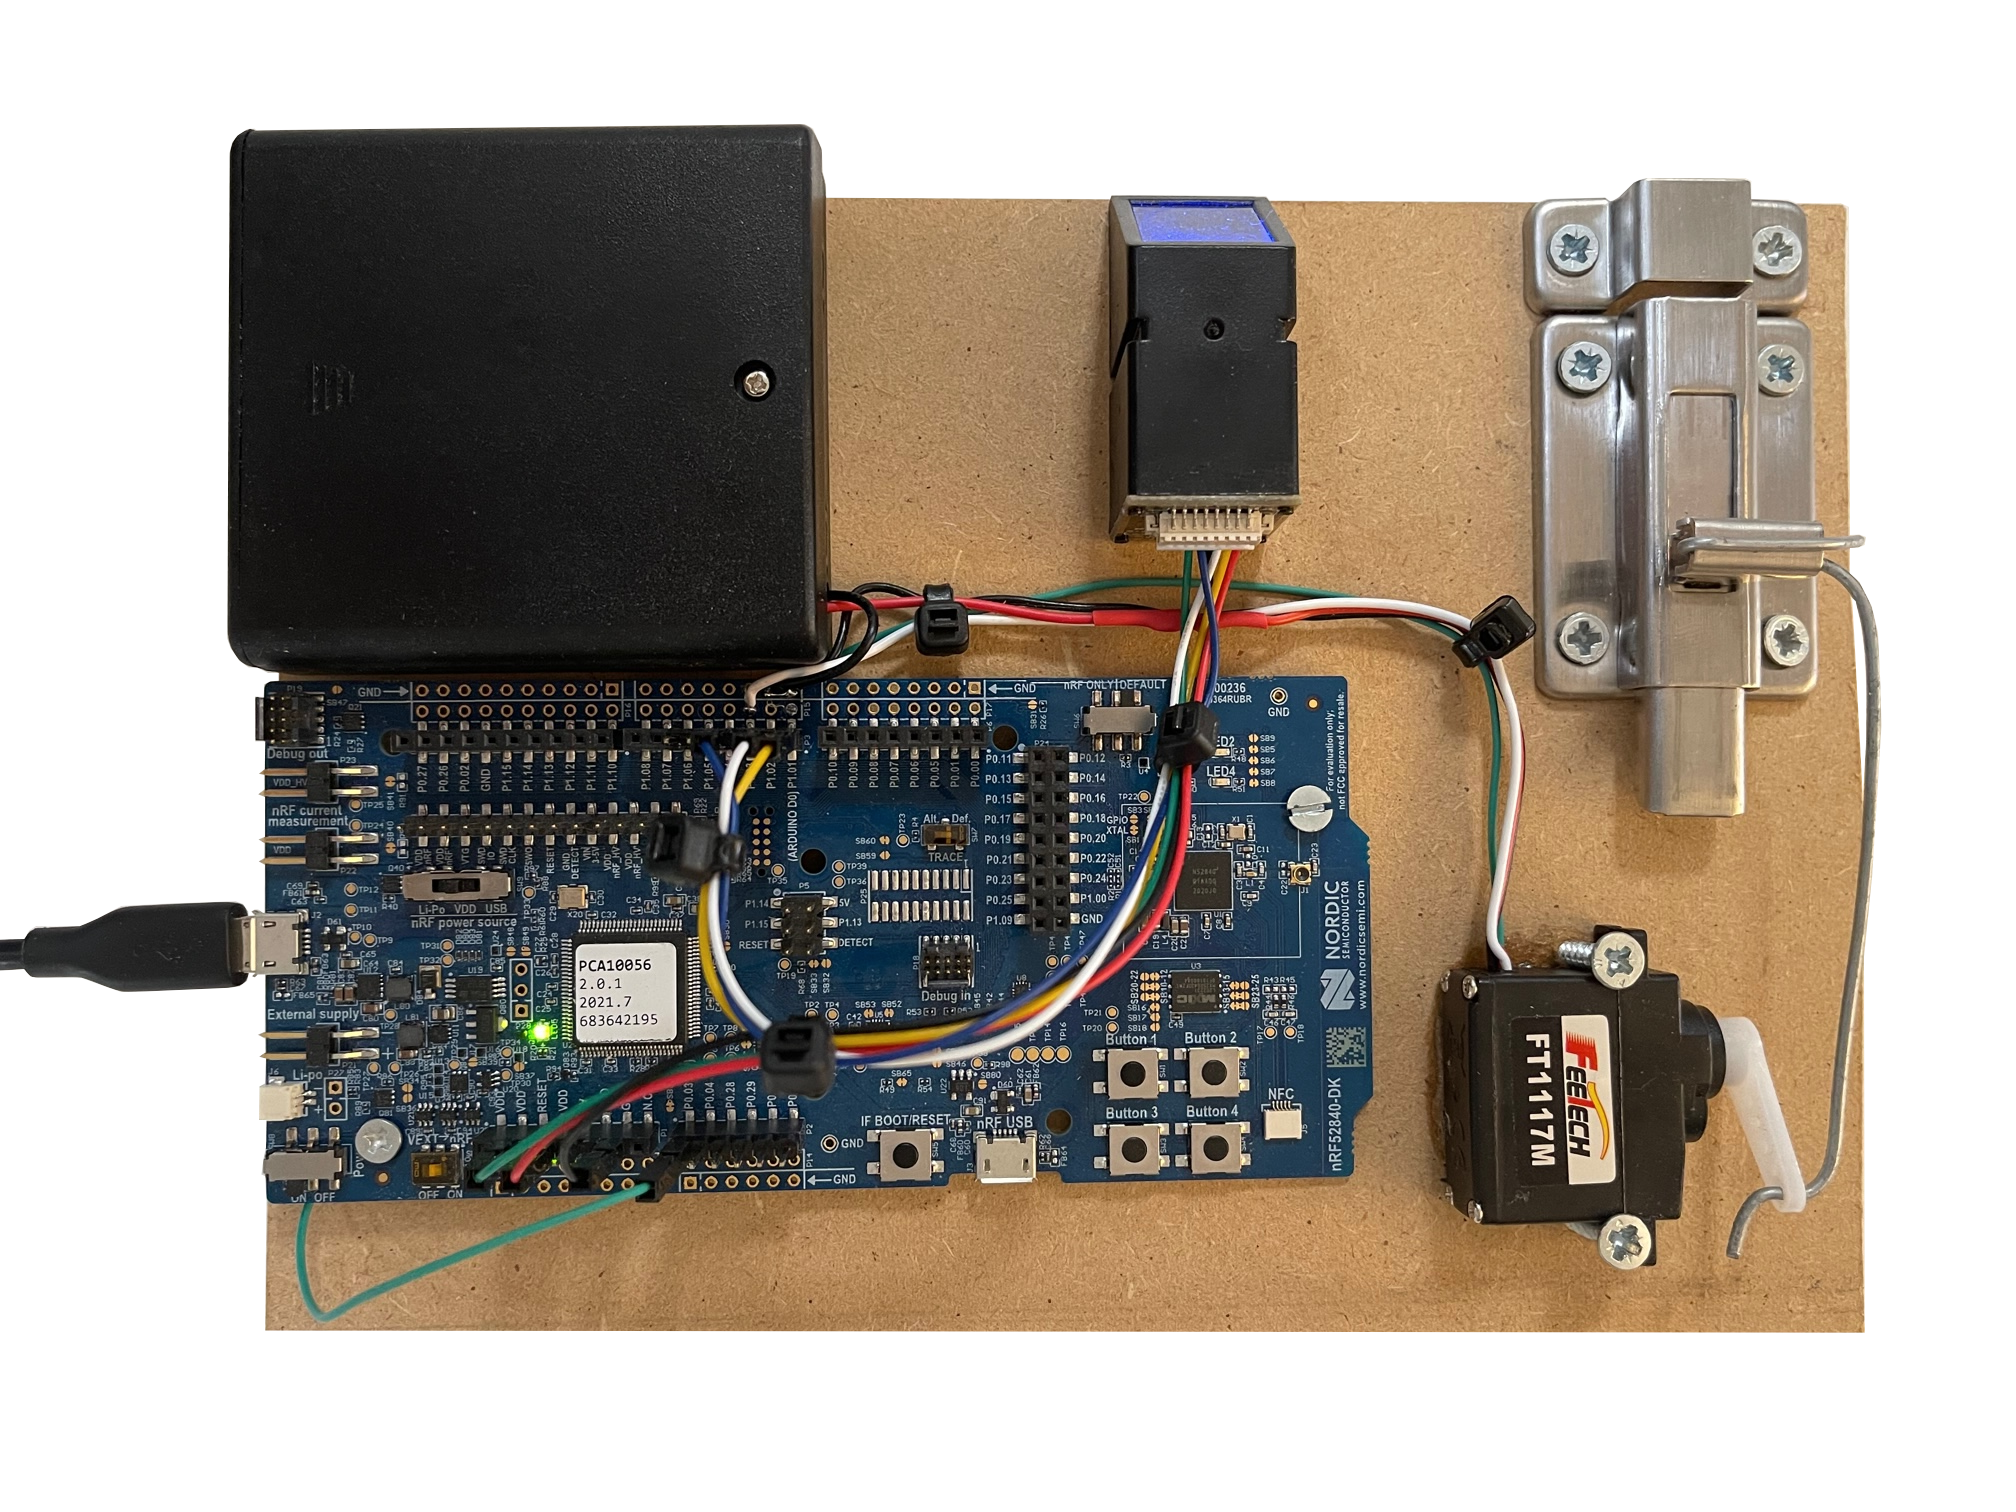
\includegraphics[scale=0.5]{smart-lock.png}
    \caption{Smart lock prototype}
  \end{figure}

  \begin{tikzpicture}[overlay,remember picture]
    \draw[->] ($(pic cs:smartlock) +(-10px,150px)$) to[out=-90,in=180] ($(pic cs:smartlock) +(25px,130px)$);
    \node[anchor=south] at ($(pic cs:smartlock) +(-10px,150px)$) {Battery};
    \draw[->] ($(pic cs:smartlock) +(-10px,20px)$) to[out=90,in=180] ($(pic cs:smartlock) +(30px,40px)$);
    \node[anchor=north] at ($(pic cs:smartlock) +(-10px,20px)$) {nRF52840DK};
    \draw[->] ($(pic cs:smartlock) +(160px,172px)$) to[out=180,in=90] ($(pic cs:smartlock) +(142px,160px)$);
    \node[anchor=west] at ($(pic cs:smartlock) +(160px,172px)$) {Fingerprint sensor};
    \draw[->] ($(pic cs:smartlock) +(260px,120px)$) to[out=90,in=0] ($(pic cs:smartlock) +(225px,135px)$);
    \node[anchor=north] at ($(pic cs:smartlock) +(260px,120px)$) {Lock};
    \draw[->] ($(pic cs:smartlock) +(260px,30px)$) to[out=90,in=0] ($(pic cs:smartlock) +(225px,50px)$);
    \node[anchor=north] at ($(pic cs:smartlock) +(260px,30px)$) {Servo};
  \end{tikzpicture}
\end{frame}

% section: device model --------------------------------------------------------

\section{Device model crash course}

\begin{frame}
  \begin{center}
    \Huge \textbf{Device model crash course}
  \end{center}
\end{frame}

\subsection{Devicetree}

\begin{frame}
  \begin{center}
    \Large \textbf{Devicetree}
  \end{center}
\end{frame}

\begin{frame}
  \frametitle{Devicetree}

  \begin{itemize}
    \item Devicetree is a hierarchical data structure inherited from
          \textbf{Linux Kernel} used to \textbf{describe hardware}
    \item \textbf{Essential} to the Zephyr device model: most devices are
          described in Devicetree
    \item There are \textbf{two} types of Devicetree \textbf{input files}:
          the \textbf{sources} and the \textbf{bindings}, which describe the
          content
    \item Devicetree in Zephyr is \textbf{parsed} at \textbf{compile time} and
          converted to \textbf{C header} files
    \item All Devicetree \textbf{information} is accessible at
          \textbf{compile time} via the \texttt{<zephyr/devicetree.h>} API
  \end{itemize}
\end{frame}

\begin{frame}[fragile]
  \frametitle{Devicetree example}

  \begin{figure}
    \begin{columns}
      \begin{column}{0.5\textwidth}
        \begin{minted}[gobble=8,fontsize=\tiny]{dts}
          /dts-v1/;

          / {
            soc {
              i2c0: i2c@40003000 {
                compatible = "nordic,nrf-twim";
                label = "I2C0";
                reg = <0x40003000 0x1000>;

                apds9960@39 {
                  compatible = "avago,apds9960";
                  label = "APDS9960";
                  reg = <0x39>;
                };

                ti_hdc@43 {
                  compatible = "ti,hdc",
                               "ti,hdc1010";
                  label = "HDC1010";
                  reg = <0x43>;
                };
              };
            };
          };
        \end{minted}
      \end{column}
      \begin{column}{0.5\textwidth}
        \scalebox{0.75}{
          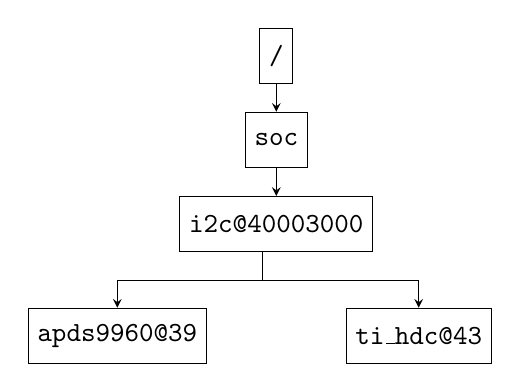
\begin{tikzpicture}
            \node [draw,
              minimum height=2em
            ] (root) {\texttt{/}};

            \node [draw,
              minimum height=2em,
              below=1em of root
            ] (soc) {\texttt{soc}};

            \node [draw,
              minimum height=2em,
              below=1em of soc
            ] (i2c) {\texttt{i2c@40003000}};

            \node [draw,
              minimum height=2em,
              below left=2em and -1em of i2c
            ] (apds9960) {\texttt{apds9960@39}};

            \node [draw,
              minimum height=2em,
              below right=2em and -1em of i2c
            ] (ti_hdc) {\texttt{ti\_hdc@43}};

            \draw[->] (root.south) -- (soc.north);
            \draw[->] (soc.south) -- (i2c.north);
            \draw[->] ([xshift=-.5em]i2c.south) -- ++(0,-1em) -| (apds9960.north);
            \draw[->] ([xshift=-.5em]i2c.south) -- ++(0,-1em) -| (ti_hdc.north);
          \end{tikzpicture}
        }
      \end{column}
    \end{columns}
    \caption{Devicetree example}
  \end{figure}
\end{frame}

\begin{frame}
  \frametitle{Important Devicetree properties}

  \begin{table}
    \centering
    \footnotesize
    \begin{tabular}{lp{0.8\textwidth}}
      \toprule
      Property            & Description                                        \\
      \midrule
      \texttt{compatible} &                                                    %
      Name of the \textbf{hardware} a node \textbf{represents}, typically
      \texttt{vendor,device}. Used to find the \textbf{bindings} for the node. \\
      \texttt{label}      &                                                    %
      \textbf{Name} of the device (unique).                                    \\
      \texttt{reg}        &                                                    %
      Information used to \textbf{address} the device (optional). Value
      meaning depends on the device. In general, it is a
      \textbf{sequence of address-length pairs.}                               \\
      \texttt{status}     &                                                    %
      \textbf{Status} of the device. \texttt{okay} (default if not specified)
      or \texttt{disabled}.                                                    \\
      \bottomrule
    \end{tabular}
    \caption{Important Devicetree properties}
  \end{table}
\end{frame}

\begin{frame}[fragile]
  \frametitle{Devicetree data types}

  \begin{table}
    \centering
    \begin{tabular}{lp{0.65\textwidth}}
      \toprule
      Type                   & Example                                      \\
      \midrule
      \texttt{string}        & \texttt{my-string = ``hello,world''}         \\
      \texttt{int}           & \texttt{my-int = <1>;}                       \\
      \texttt{boolean}       & \texttt{enable-my-feature;}                  \\
      \texttt{array}         & \texttt{my-ints = <0xdeadbeef 1234 0>;}      \\
      \texttt{uint8-array}   & \texttt{my-bytes = [00 01 ab];}              \\
      \texttt{string-array}  & \texttt{my-strings = ``str1'', ``str2'';}    \\
      \texttt{phandle}       & \texttt{my-uart = <\&uart0>;}                \\
      \texttt{phandles}      & \texttt{my-uarts = <\&uart0 \&uart1>;}       \\
      \texttt{phandle-array} & \texttt{io-channels = <\&adc 0>, <\&adc 1>;} \\
      \bottomrule
    \end{tabular}
    \caption{Devicetree data types}
  \end{table}
\end{frame}

\begin{frame}[fragile]
  \frametitle{Devicetree instances}

  \begin{itemize}
    \item Multiple \textbf{instances} of the same device can be defined in
          Devicetree, each with its \textbf{own} properties
  \end{itemize}

  \begin{listing}[H]
    \begin{minted}[gobble=4,fontsize=\tiny]{dts}
      / {
        /* one instance of 'nordic,nrf-twim' */
        i2c0: i2c@40003000 {
          compatible = "nordic,nrf-twim";
          label = "I2C_0";
          reg = <0x40003000 0x1000>;
          clock-frequency = <I2C_BITRATE_STANDARD>;
        };

        /* another instance of 'nordic,nrf-twim' */
        i2c1: i2c@40004000 {
          compatible = "nordic,nrf-twim"
          label = "I2C_1";
          reg = <0x40004000 0x1000>;
          clock-frequency = <I2C_BITRATE_FAST>;
        };
      };
    \end{minted}
    \caption{\texttt{i2c0} and \texttt{i2c1} are two instances of
      \texttt{nordic,nrf-twim}}
  \end{listing}
\end{frame}

\begin{frame}
  \frametitle{Devicetree composition}

  \begin{itemize}
    \item The \textbf{final} Devicetree source is a result of
          \textbf{overlaying} multiple sources: SoC sources, board sources,
          application overlays with overrides, etc.
  \end{itemize}

  \begin{figure}
    \centering
    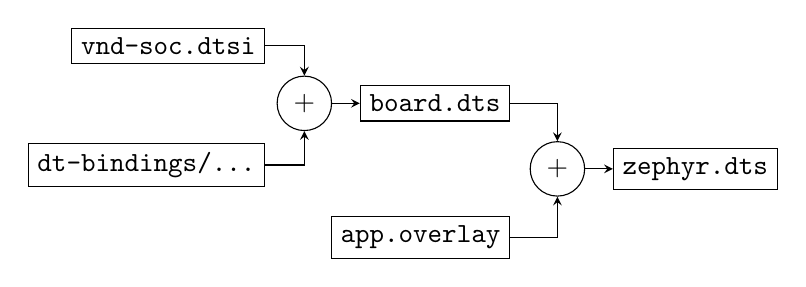
\begin{tikzpicture}
      \node [draw
      ] (zephyr) {\texttt{zephyr.dts}};
      \node [draw,
        circle,
        left=1em of zephyr
      ] (addfinal) {+};
      \node [draw,
        above left=1em and 1em of addfinal
      ] (board) {\texttt{board.dts}};
      \node [draw,
        circle,
        left=1em of board
      ] (addboard) {+};
      \node [draw,
        above left=1em of addboard
      ] (soc) {\texttt{vnd-soc.dtsi}};
      \node [draw,
        below left=1em of addboard
      ] (bindings) {\texttt{dt-bindings/...}};
      \node [draw,
        below left=1em and 1em of addfinal
      ] (app) {\texttt{app.overlay}};

      \draw[->] (addfinal.east) -- (zephyr.west);
      \draw[->] (board.east) -| (addfinal.north);
      \draw[->] (addboard.east) -- (board.west);
      \draw[->] (soc.east) -| (addboard.north);
      \draw[->] (bindings.east) -| (addboard.south);
      \draw[->] (app.east) -| (addfinal.south);
    \end{tikzpicture}
    \caption{Devicetree composition example}
  \end{figure}
\end{frame}

\begin{frame}[fragile]
  \frametitle{Devicetree composition: example}

  \begin{listing}[H]
    \begin{columns}
      \begin{column}{0.5\textwidth}
        \begin{minted}[gobble=8,fontsize=\scriptsize]{dts}
          /* vnd-soc.dtsi */
          \ {
            soc {
              uart0: uart@abcd1234 {
                compatible = "vnd,uart";
                reg = <0xabcd1234 0x1000>;
                status = "disabled";
              };
            };
          };
        \end{minted}
        \begin{minted}[gobble=8,fontsize=\scriptsize]{dts}
          /* board.dts */
          #include <vnd-soc.dtsi>

          &uart0 {
            status = "okay";
            current-speed = <9600>;
          }
        \end{minted}
      \end{column}
      \begin{column}{0.5\textwidth}
        \begin{minted}[gobble=8,fontsize=\scriptsize]{dts}
          /* zephyr.dts (final) */
          \ {
            soc {
              uart0: uart@abcd1234 {
                compatible = "vnd,uart";
                reg = <0xabcd1234 0x1000>;
                status = "okay";
                current-speed = <9600>;
              };
            };
          };
        \end{minted}
      \end{column}
    \end{columns}
    \caption{Devicetree composition example}
  \end{listing}

  \begin{tikzpicture}[overlay,remember picture]
    \node[draw,
      circle,
      fill=white
    ] (add) at (2.5,4.25) {+};
    \draw[->] (add.east) to[out=0,in=180] (5.7,4.25);
  \end{tikzpicture}
\end{frame}

\begin{frame}[fragile]
  \frametitle{Devicetree bindings}

  \begin{itemize}
    \item \textbf{Content} of Devicetree, including data types, is
          \textbf{described} in \textbf{binding} files
    \item Binding files are used by the Devicetree parser to
          \textbf{validate content}
    \item Binding files are written in \textbf{YAML}, structure custom to
          Zephyr
  \end{itemize}

  \begin{listing}[H]
    \begin{columns}
      \begin{column}{0.5\textwidth}
        \begin{minted}[fontsize=\tiny,escapeinside=??]{yaml}
        description: ...

        compatible: vnd,dev?\tikzmark{bindingcompat}?

        include: base.yaml?\tikzmark{bindingbaseprop}?

        properties:
          foo:?\tikzmark{bindingprop}?
            type: int
            required: true
      \end{minted}
      \end{column}
      \begin{column}{0.5\textwidth}
        \begin{minted}[fontsize=\tiny,escapeinside=??]{dts}
        / {
          dev0: dev@deadbeef {
            ?\tikzmark{dtcompat}?compatible = "vnd,dev"
            ?\tikzmark{dtbaseprop1}?label = "DEV0";
            ?\tikzmark{dtbaseprop2}?reg = <0xdeadbeef>;
            ?\tikzmark{dtprop}?foo = <7>;
          };
        };
      \end{minted}
      \end{column}
    \end{columns}
    \caption{Binding file (left) and Devicetree source (right)}
  \end{listing}

  \begin{tikzpicture}[overlay,remember picture]
    \draw[->] (pic cs:dtcompat) to[out=180,in=0] (pic cs:bindingcompat);
    \draw[->] (pic cs:dtbaseprop1) to[out=180,in=0] (pic cs:bindingbaseprop);
    \draw[->] (pic cs:dtbaseprop2) to[out=180,in=0] (pic cs:bindingbaseprop);
    \draw[->] (pic cs:dtprop) to[out=180,in=0] (pic cs:bindingprop);
  \end{tikzpicture}
\end{frame}

\begin{frame}
  \frametitle{Devicetree bindings composition}

  \begin{itemize}
    \item Devicetree bindings can \textbf{include} other base files, allowing to
          \textbf{re-use} common properties
  \end{itemize}

  \begin{figure}
    \centering
    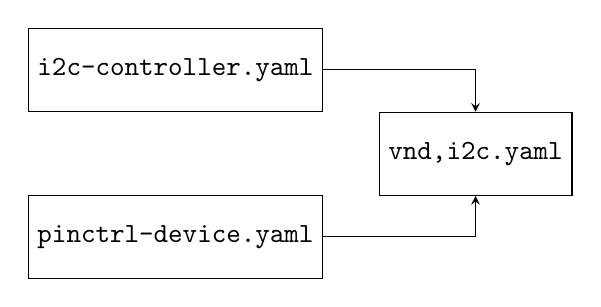
\begin{tikzpicture}
      \node [draw,
        minimum height=3em
      ] (base) {\texttt{i2c-controller.yaml}};

      \node [draw,
        minimum height=3em,
        below=3em of base
      ] (display) {\texttt{pinctrl-device.yaml}};

      \node [draw,
        minimum height=3em,
        below right=0 and 2em of base
      ] (final) {\texttt{vnd,i2c.yaml}};

      \draw[->] (base.east) -| (final.north);
      \draw[->] (display.east) -| (final.south);
    \end{tikzpicture}
    \caption{An I2C controller binding includes \texttt{i2c-controller.yaml}
      (e.g.\ for bus address/size, \texttt{clock-frequency}) and
      \texttt{pinctrl-device.yaml} (e.g.\ for \texttt{pinctrl-0})}
  \end{figure}
\end{frame}

\begin{frame}
  \frametitle{Devicetree output}

  \begin{itemize}
    \item Devicetree is \textbf{converted} to a \textbf{C header} with a series
          of \textbf{C definitions} at compile time: \textbf{ZERO OVERHEAD!}
    \item Devicetree does not \textbf{\textit{exist}} after code is compiled,
          only stored information will \textit{survive}.
  \end{itemize}

  \begin{figure}
    \centering
    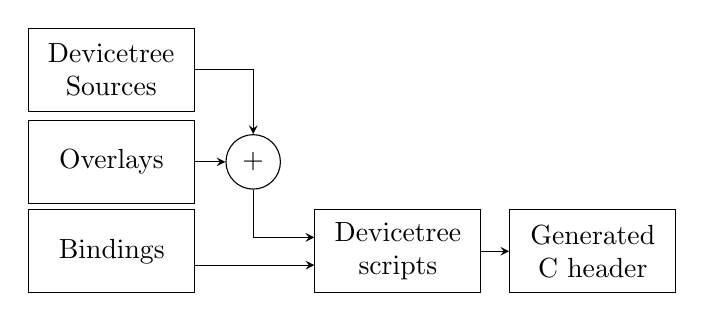
\begin{tikzpicture}[
        block/.style={
            draw,
            minimum height=3em,
            minimum width=6em,
            align=center,
          },
      ]
      \node [
        block
      ] (code) {Generated\\ C header};
      \node [
        block,
        left=1em of code
      ] (scripts) {Devicetree\\ scripts};
      \node [
        draw,
        circle,
        above left=1em and 1.5em of scripts
      ] (add) {+};
      \node [
        block,
        above left=1.1em and 1.4em of add,
      ] (sources) {Devicetree\\ Sources};
      \node [
        block,
        left=1.1em and 1.1em of add
      ] (overlays) {Overlays};
      \node [
        block,
        left=4.3em of scripts
      ] (bindings) {Bindings};

      \draw[->] (scripts.east) -- (code.west);
      \draw[->] (add.south) |- ([yshift=0.5em]scripts.west);
      \draw[->] (sources.east) -| (add.north);
      \draw[->] (overlays.east) -- (add.west);
      \draw[->] ([yshift=-0.5em]bindings.east) -- ([yshift=-0.5em]scripts.west);
    \end{tikzpicture}
    \caption{Generation of C header from Devicetree}
  \end{figure}
\end{frame}

\begin{frame}[fragile]
  \frametitle{Devicetree output: example}

  The \texttt{current-speed} property for the UART device

  \begin{minted}[fontsize=\tiny]{dts}
    \ {
      soc {
        uart0: uart@abcd1234 {
          ...
          current-speed = <9600>;
        };
      };
    };
  \end{minted}

  Becomes\dots

  \begin{minted}[fontsize=\tiny]{c}
    #define DT_N_S_soc_S_uart_abdc1234_P_current_speed 9600
  \end{minted}

  \vspace{1em}

  \textbf{NOTE:} Generated definitions must never be used directly in code!
\end{frame}

\begin{frame}
  \frametitle{Accessing Devicetree from C}

  \begin{itemize}
    \item Devicetree information is accessed using the
          \textbf{\texttt{<zephyr/devicetree.h>} API}, \textbf{never} using
          generated definitions
    \item Devicetree API is \textbf{macro-based}, built upon C-preprocessor
          \textbf{token concatenation}
    \item Information about a particular node, can be obtained using a
          \textbf{node identifier}
  \end{itemize}
\end{frame}

\begin{frame}[fragile]
  \frametitle{How to obtain a node identifier}

  \begin{listing}[H]
    \begin{columns}
      \begin{column}{0.5\textwidth}
        \begin{minted}[gobble=8,fontsize=\tiny]{dts}
          /dts-v1/;

          / {

            chosen {
              zephyr,console = &uart0;
            };

            aliases {
              my-uart = &uart0;
            };

            soc {
              uart0: uart@abcd1234 {
                compatible = "vnd,soc-uart";
                reg = <0xabcd1234 0x1000>;
                current-speed = <9600>;
              };
            };
          };
      \end{minted}
      \end{column}
      \begin{column}{0.5\textwidth}
        \begin{minted}[gobble=8,fontsize=\tiny]{c}
          /* by full path */
          DT_PATH(soc, uart_abcd1234)

          /* by node label */
          DT_NODELABEL(uart0)

          /* by using an alias
           * useful for generic samples
           */
          DT_ALIAS(my_uart)

          /* by using a choice
           * typically used by subsystems
           */
          DT_CHOSEN(zephyr_console)

          /* by specifying an instance number
           * of a given compatible, e.g. 0
           */
          DT_INST(0, vnd_soc_uart)
      \end{minted}
      \end{column}
    \end{columns}
    \caption{Examples on how to obtain the node identifier for the
      \texttt{uart@abcd1234} node}
  \end{listing}
\end{frame}

\begin{frame}[fragile]
  \frametitle{Accessing Devicetree from C:\ examples}

  \begin{listing}[H]
    \begin{columns}
      \begin{column}{0.5\textwidth}
        \begin{minted}[escapeinside=??,fontsize=\tiny]{dts}
  /dts-v1/;

  / {
      i2c0: i2c@abcd1234 {?\tikzmark{dt_i2c0}?
        ...
        sensor0: sensor@ff {
          compatible = "vnd,mysensor";
          reg = <0xff>;?\tikzmark{dt_reg}?
          int-gpios = <&gpio0?\tikzmark{dt_gpio0}? 1?\tikzmark{dt_pin}?
                        GPIO_ACTIVE_HIGH>;
          sample-freq = <1000>;?\tikzmark{dt_samplefreq}?
        };
      };
    };
  };
      \end{minted}
      \end{column}
      \begin{column}{0.5\textwidth}
        \begin{minted}[escapeinside=??,fontsize=\tiny]{c}
  /* use node label to obtain sensor node
   * identifier
   */
  #define SENSOR_0 DT_NODELABEL(sensor0)

  /* expands to 0xff */
  ?\tikzmark{c_reg}?DT_REG_ADDR(SENSOR_0)

  /* expands to gpio0 node identifier */
  ?\tikzmark{c_gpio0}?DT_PHANDLE(SENSOR_0, int_gpios)
  /* equivalent (GPIO specific helpers) */
  ?\tikzmark{c_gpio0_gpio}?DT_GPIO_CTLR(SENSOR_0, int_gpios)

  /* expands to 1 (pin cell) */
  ?\tikzmark{c_pin}?DT_PHA(SENSOR_0, int_gpios, pin)
  /* equivalent (GPIO specific helpers) */
  ?\tikzmark{c_pin_gpio}?DT_GPIO_PIN(SENSOR_0, int_gpios)

  /* expands to 1000 */
  ?\tikzmark{c_samplefreq}?DT_PROP(SENSOR_0, sample_freq)
      \end{minted}
      \end{column}
    \end{columns}
    \caption{Examples on how to access Devicetree information}
  \end{listing}

  \centering\faBook~\href{
    https://docs.zephyrproject.org/latest/build/dts/api/index.html}{
    https://docs.zephyrproject.org/latest/build/dts/api/index.html
  }

  \begin{tikzpicture}[overlay,remember picture]
    \draw[->] (pic cs:c_reg) to[out=180,in=90] ($(pic cs:dt_reg) +(-2.5ex,0.3em)$);
    \draw[->] (pic cs:c_gpio0) to[out=180,in=90] ($(pic cs:dt_gpio0) +(-2.5ex,0.3em)$);
    \draw[->] (pic cs:c_gpio0_gpio) to[out=180,in=90] ($(pic cs:dt_gpio0) +(-2.5ex,0.3em)$);
    \draw[->] (pic cs:c_pin) to[out=180,in=0] (pic cs:dt_pin);
    \draw[->] (pic cs:c_pin_gpio) to[out=180,in=0] (pic cs:dt_pin);
    \draw[->] (pic cs:c_samplefreq) to[out=180,in=0] (pic cs:dt_samplefreq);
  \end{tikzpicture}
\end{frame}

\begin{frame}[fragile]
  \frametitle{Instance-based Devicetree API}

  \begin{itemize}
    \item It is often necessary to write code
          \textbf{generic to any device instance}, specially in a
          \textbf{driver context}
    \item Most Devicetree APIs have their \textbf{instance-based version}, e.g.\
          for \texttt{DT\_PROP} we have \texttt{DT\_INST\_PROP}
    \item Instance-based macros \textbf{rely} on \texttt{DT\_DRV\_COMPAT} being
          \textbf{defined} to the compatible implemented by the driver
  \end{itemize}

  \begin{listing}[H]
    \begin{minted}[gobble=4,fontsize=\tiny]{c}
      /* we're working with vnd,mysensor compatible */
      #define DT_DRV_COMPAT vnd_mysensor

      /* obtain 'sample-freq' property value for instance 0
       * of vnd,mysensor
       */
      uint32_t sample_freq = DT_INST_PROP(0, sample_freq)
    \end{minted}
    \caption{Example of instance-based Devicetree API}
  \end{listing}
\end{frame}

\subsection{Zephyr devices}

\begin{frame}
  \begin{center}
    \Large \textbf{Zephyr devices}
  \end{center}
\end{frame}

\begin{frame}
  \frametitle{Zephyr devices}

  \begin{itemize}
    \item Zephyr devices are represented by \mintinline{c}{struct device},
          defined in \texttt{<zephyr/device.h>}
    \item \mintinline{c}{struct device} just holds a series of
          \textbf{references} to resources \textbf{defined by drivers} or
          \textbf{defined internally} by the device definition macros
    \item Devices are \textbf{defined} in \textbf{ROM} by a series of
          \textbf{macros}:
          \begin{itemize}
            \item \texttt{DEVICE\_DEFINE}: Non-Devicetree devices
            \item \texttt{DEVICE\_DT\_DEFINE}/\texttt{DEVICE\_DT\_INST\_DEFINE}:
                  Devicetree-based devices
          \end{itemize}
    \item Devices are \textbf{automatically initialized} at boot time, before
          \texttt{main} is reached
    \item Devices are \textbf{initialized} in a specific \textbf{order},
          determined by a \textbf{level} and a manually defined
          \textbf{priorities}
  \end{itemize}
\end{frame}

\begin{frame}[fragile]
  \frametitle{Device structure}

  \begin{listing}[H]
    \begin{minted}[fontsize=\tiny]{c}
      struct device {
        const char *name;
        const void *config;
        void * const data;
        const void *api;
        ...
      };
    \end{minted}
    \caption{Core \mintinline{c}{struct device} members}
  \end{listing}

  \begin{table}
    \centering
    \footnotesize
    \begin{tabular}{lp{0.8\textwidth}}
      \toprule
      Field           & Purpose                                            \\
      \midrule
      \texttt{name}   &                                                    %
      Device name (unique), corresponds to the \textbf{\texttt{label}}
      property for Devicetree devices                                      \\
      \texttt{config} &                                                    %
      Reference to \textbf{read-only configuration} set at
      \textbf{compile time}, tipically used to store Devicetree properties \\
      \texttt{data}   &                                                    %
      Reference to device \textbf{data} that needs to be modified at
      \textbf{runtime}, e.g.\ counter, state, etc.                         \\
      \texttt{api}    &                                                    %
      Reference to the device \textbf{API operations}                      \\
      \bottomrule
    \end{tabular}
    \caption{Core \mintinline{c}{struct device} members description}
  \end{table}
\end{frame}

\begin{frame}[fragile]
  \frametitle{Device definition}
  \begin{listing}[H]
    \begin{minted}[gobble=4,fontsize=\tiny]{c}
      /* define a device given an instance number */
      DEVICE_DT_INST_DEFINE(
        inst,                 /* Devicetree instance number */
        init_fn,              /* Initialization function */
        pm_device,            /* Power management resources (optional) */
        data_ptr,             /* Reference to instance data */
        config_ptr,           /* Reference to instance configuration */
        level,                /* Initialization level (e.g. POST_KERNEL) */
        prio,                 /* Initialization priority (0-99) */
        api_ptr,              /* Reference to API operations */
      );
    \end{minted}
    \caption{Definition of a Devicetree device\footnotemark}
  \end{listing}

  \footnotetext{\texttt{DEVICE\_DT\_DEFINE} is also available if using a DT node
    identifier instead of an instance number}
\end{frame}

\subsection{Example device driver}

\begin{frame}
  \begin{center}
    \Large \textbf{Example device driver}
  \end{center}
\end{frame}

\begin{frame}[fragile]
  \frametitle{Device driver example: bindings}

  \begin{listing}[H]
    \begin{minted}[gobble=4,fontsize=\tiny]{yaml}
      description: ...

      compatible: vnd,mysensor

      include: base.yaml

      properties:
        reg:
          required: true

        int-gpios:
          type: phandle-array
          required: true

        sample-freq:
          type: int
          required: true
    \end{minted}
    \caption{Devicetree bindings for \texttt{vnd,mysensor}, tipically in
      \texttt{dts/bindings/...}}
  \end{listing}
\end{frame}

\begin{frame}[fragile]
  \frametitle{Device driver example: source (I)}

  \begin{listing}[H]
    \begin{minted}[gobble=4,fontsize=\tiny]{c}
      /* tells DT INST based macros which compatible to use
       * tipically defined at the top, but can be defined
       * anywhere before using DT INST based macros
       */
      #define DT_DRV_COMPAT vnd_mysensor
    \end{minted}
    \caption{Definition of driver compatible}
  \end{listing}
\end{frame}

\begin{frame}[fragile]
  \frametitle{Device driver example: source (II)}

  \begin{listing}[H]
    \begin{minted}[gobble=4,fontsize=\tiny]{c}
      /* driver configuration (immutable)
       * tipically information retrieved from Devicetree
       */
      struct mysensor_config {
        uint8_t reg;
        struct gpio_dt_spec int_gpio;
        uint32_t sample_freq;
      }

      /* driver data (mutable) */
      struct mysensor_data {
        uint8_t buf[32];
        struct k_msgq queue;
      };
    \end{minted}
    \caption{Definition of driver configuration and data structures}
  \end{listing}
\end{frame}

\begin{frame}[fragile]
  \frametitle{Device driver example: source (III)}

  \begin{listing}[H]
    \begin{minted}[gobble=4,fontsize=\tiny]{c}
      static int mysensor_sample_fetch(const struct device *dev, ...)
      {
        /* implementation of API sample_fetch operation */
      }
      ...

      static const struct sensor_driver_api mysensor_api = {
        .sample_fetch = mysensor_sample_fetch,
        ...
      };
    \end{minted}
    \caption{Definition driver API operations (sensor API here)}
  \end{listing}

  \begin{listing}[H]
    \begin{minted}[gobble=4,fontsize=\tiny]{c}
      static int mysensor_init(const struct device *dev)
      {
        /* initialize driver (e.g. check for dependent devices readiness) */
      }
    \end{minted}
    \caption{Definition of driver initialization function}
  \end{listing}
\end{frame}

\begin{frame}[fragile]
  \frametitle{Device driver example: source (IV)}

  \begin{listing}[H]
    \begin{minted}[gobble=4,fontsize=\tiny]{c}
      /* macro to define an instance of our device
       * this code applies to any instance, so we're using DT_INST_* macros
       */
      #define MYSENSOR_DEFINE(i)                                             \
        static const struct config##i = {                                    \
          .reg = DT_REG_INST_ADDR(i),                                        \
          .int_gpio = GPIO_DT_SPEC_INST_GET(i, int_gpios),                   \
          .sample_freq = DT_INST_PROP(i, sample_freq),                       \
        };                                                                   \
                                                                             \
        static struct mysensor_data data##i;                                 \
                                                                             \
        DEVICE_DT_INST_DEFINE(i, mysensor_init, NULL, &data##i, &config##i   \
                              POST_KERNEL, CONFIG_SENSOR_PRIORITY,           \
                              &mysensor_api);

      /* expands MYSENSOR_DEFINE for each device in DT with compatible
       * vnd,mysensor (defined by DT_DRV_COMPAT) and status "okay"
       */
      DT_INST_FOREACH_STATUS_OKAY(MYSENSOR_DEFINE)
    \end{minted}
    \caption{Device driver definition, multi-instance capable}
  \end{listing}
\end{frame}

\begin{frame}[fragile]
  \frametitle{Device driver example: Devicetree instantiation}

  \begin{listing}[H]
    \begin{minted}[gobble=4,fontsize=\tiny]{dts}
      /dts-v1/;

      / {
          i2c0: i2c@abcd1234 {
            ...
            accel: sensor@ff {
              compatible = "vnd,mysensor";
              label = "ACCEL"
              reg = <0xff>;
              int-gpios = <&gpio0 1 GPIO_ACTIVE_HIGH>;
              sample-freq = <1000>;
            };
          };
        };
      };
    \end{minted}
    \caption{Instantiation of \texttt{vnd,mysensor} in Devicetree}
  \end{listing}
\end{frame}

\begin{frame}[fragile]
  \frametitle{Obtaining references to devices}

  \begin{itemize}
    \item \textbf{References} to \textbf{Devicetree} devices can be obtained
          at \textbf{compile-time} using \texttt{DEVICE\_DT\_GET} family of
          macros
    \item \textbf{References} can also be obtained at \textbf{runtime} by
          name, using \texttt{device\_get\_binding} (rarely needed nowadays)
  \end{itemize}

  \begin{listing}[H]
    \begin{minted}[gobble=4,fontsize=\tiny]{c}
      /* get reference to a device using a node identifier */
      const struct device *dev = DEVICE_DT_GET(DT_NODELABEL(accel));

      /* get reference to a device using a node identifier, NULL if none */
      const struct device *dev = DEVICE_DT_GET_OR_NULL(DT_NODELABEL(accel));

      /* obtain one reference of the vnd,my-sensor compatible, NULL if none */
      const struct device *dev = DEVICE_DT_GET_ANY(vnd_my_sensor);

      /* obtain one reference of the vnd,my-sensor compatible */
      const struct device *dev = DEVICE_DT_GET_ONE(vnd_my_sensor);
  
      /* get reference to a device at runtime, using name lookup */
      const struct device *dev = device_get_binding("ACCEL");
    \end{minted}
    \caption{Examples on how to obtain device references}
  \end{listing}
\end{frame}

% section: implementing a sensor driver ----------------------------------------

\section{Implementing a sensor driver}

\begin{frame}
  \begin{center}
    \Huge \textbf{Implementing a\\sensor driver}
  \end{center}
\end{frame}

\subsection{JM-101 fingerprint sensor}

\begin{frame}
  \begin{center}
    \Large \textbf{JM-101 fingerprint sensor}
  \end{center}
\end{frame}

\begin{frame}
  \frametitle{JM-101 fingerprint sensor}

  \begin{itemize}
    \item JM-101 is a \textbf{fingerprint} sensor manufactured by
          \href{www.zeantec.com}{Hangzhou Zhean Technology Co. Ltd.}
    \item Based on \textbf{Synodata GC0328} firmware, same as many clones
    \item Not strictly a sensor, but a \textbf{biometric} device
    \item Allows to \textbf{save} and \textbf{verify} fingerprints
    \item \textbf{UART} based communications, includes a \textbf{touch output}
  \end{itemize}

  \begin{figure}
    \centering
    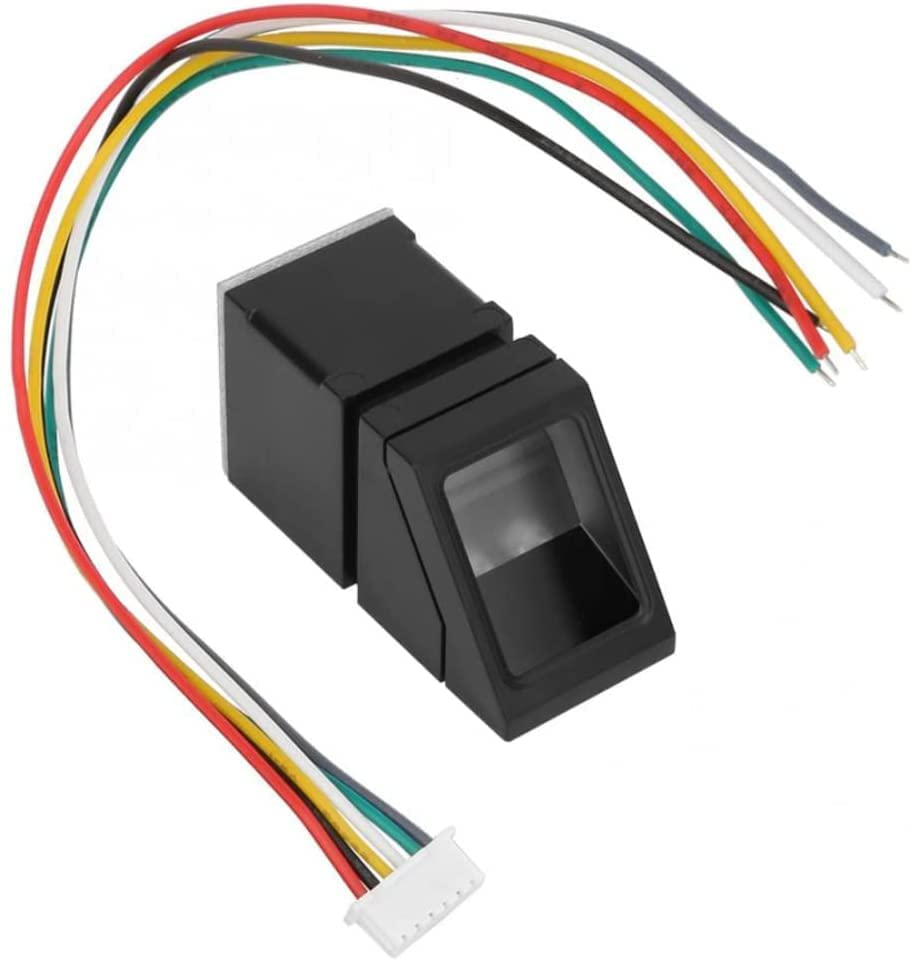
\includegraphics[scale=0.1]{fingerprint-sensor.jpg}
    \caption{JM-101 fingerprint sensor}
  \end{figure}
\end{frame}

\begin{frame}
  \frametitle{JM-101 fingerprint sensor: wiring example}

  \begin{figure}
    \centering
    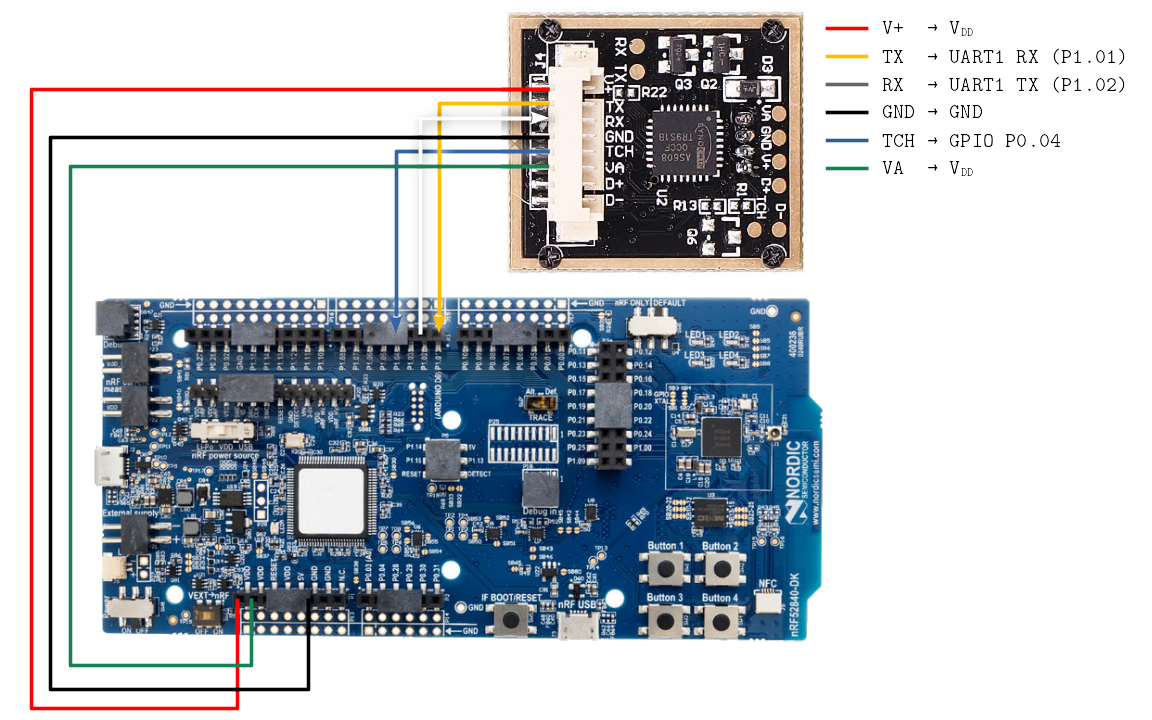
\includegraphics[scale=0.25]{fingerprint-sensor-wiring.png}
    \caption{Wiring diagram for JM-101 fingerprint sensor and nRF52840DK}
  \end{figure}
\end{frame}

\begin{frame}
  \frametitle{JM-101 fingerprint sensor: communications (I)}

  \begin{itemize}
    \item All data is transmitted \textbf{big-endian}
    \item Communications are \textbf{synchronous}
    \item Communication \textbf{parameters} are:
  \end{itemize}

  \begin{table}
    \centering
    \begin{tabular}{ll}
      \toprule
      Parameter & Value \\
      \midrule
      Baudrate  & 57600 \\
      Data bits & 8     \\
      Parity    & None  \\
      Stop bits & 2     \\
      \bottomrule
    \end{tabular}
    \caption{Serial communications parameters}
  \end{table}
\end{frame}

\begin{frame}
  \frametitle{JM-101 fingerprint sensor: communications (II)}

  \begin{itemize}
    \item Actions are triggered by MCU sending command packets
    \item Packet is structured as follows:
  \end{itemize}

  \begin{table}
    \centering
    \footnotesize
    \begin{tabular}{ccccccc}
      \toprule
      Header & Address       & Identifier & Length & Command      & Data          & Checksum                          \\
      \midrule
      2b     & 4b            & 1b         & 2b     & 1b           & Nb            & 2b                                \\
      \midrule
      EF01H  & \texttt{ADDR} & 01H        & N + 3  & \texttt{CMD} & \texttt{DATA} & $\sum_{i=6}^{10+N} \textrm{p}[i]$ \\
      \bottomrule
    \end{tabular}
  \end{table}

  \begin{itemize}
    \item Where:
          \begin{itemize}
            \item \texttt{ADDR} is the address value, tipically FFFFFFFFH
            \item \texttt{CMD} is the command, e.g.\ 31H for
                  \texttt{PS\_AutoEnroll}
            \item \texttt{DATA} are the N bytes of payload
          \end{itemize}
  \end{itemize}
\end{frame}

\begin{frame}
  \frametitle{JM-101 fingerprint sensor: communications (III)}

  \begin{itemize}
    \item Sensor responds to commands with a response packet/s
    \item Packet is structured as follows:
  \end{itemize}

  \begin{table}
    \centering
    \footnotesize
    \begin{tabular}{ccccccc}
      \toprule
      Header & Address       & Identifier & Length & Result       & Data          & Checksum                          \\
      \midrule
      2b     & 4b            & 1b         & 2b     & 1b           & Nb            & 2b                                \\
      \midrule
      EF01H  & \texttt{ADDR} & 07H        & N + 3  & \texttt{RES} & \texttt{DATA} & $\sum_{i=6}^{10+N} \textrm{p}[i]$ \\
      \bottomrule
    \end{tabular}
  \end{table}

  \begin{itemize}
    \item Where:
          \begin{itemize}
            \item \texttt{ADDR} is the address value, tipically FFFFFFFFH
            \item \texttt{RES} is the command result, e.g.\ 00H = success
            \item \texttt{DATA} are the N bytes of payload
          \end{itemize}
  \end{itemize}
\end{frame}

\begin{frame}[fragile]
  \frametitle{JM-101 fingerprint sensor: communications (IV)}

  \vspace{4em}

  \begin{listing}[H]
    \begin{minted}[fontsize=\footnotesize,escapeinside=??]{text}
      MCU |-------------------------------------| SENSOR
       -> | ?\tikzmark{header}?ef 01 ?\tikzmark{addr}?ff ff ff ff ?\tikzmark{id}?01 ?\tikzmark{len}?00 03 ?\tikzmark{cmd}?0d ?\tikzmark{sum}?00 11 |
          | ef 01 ff ff ff ff 07 00 03 00 00 0a | <-
    \end{minted}
    \caption{Communications sequence for \texttt{PS\_Empty} (\texttt{0DH})
      command}
  \end{listing}

  \begin{tikzpicture}[overlay,remember picture]
    \draw[->] ($(pic cs:header) +(-3ex,3em)$) to[out=0,in=90] ($(pic cs:header) +(2.5ex,0.5em)$);
    \node[anchor=east] at ($(pic cs:header) +(-3ex,3em)$) {Header};
    \draw[->] ($(pic cs:addr) +(-3ex,4.5em)$) to[out=0,in=90] ($(pic cs:addr) +(5ex,0.5em)$);
    \node[anchor=east] at ($(pic cs:addr) +(-3ex,4.5em)$) {Address};
    \draw[->] ($(pic cs:id) +(-8ex,6em)$) to[out=0,in=90] ($(pic cs:id) +(1ex,0.5em)$);
    \node[anchor=east] at ($(pic cs:id) +(-8ex,6em)$) {Identifier};
    \draw[->] ($(pic cs:len) +(10ex,6em)$) to[out=180,in=90] ($(pic cs:len) +(2.5ex,0.5em)$);
    \node[anchor=west] at ($(pic cs:len) +(10ex,6em)$) {Length};
    \draw[->] ($(pic cs:cmd) +(7ex,4.5em)$) to[out=180,in=90] ($(pic cs:cmd) +(1ex,0.5em)$);
    \node[anchor=west] at ($(pic cs:cmd) +(7ex,4.5em)$) {Command/Response};
    \draw[->] ($(pic cs:sum) +(5.5ex,3em)$) to[out=180,in=90] ($(pic cs:sum) +(2.5ex,0.5em)$);
    \node[anchor=west] at ($(pic cs:sum) +(5.5ex,3em)$) {Checksum};
  \end{tikzpicture}
\end{frame}

\begin{frame}
  \frametitle{JM-101 operation details: verify (I)}

  \begin{itemize}
    \item Fingerprint verification sequence is triggered by
          \textbf{\texttt{PS\_AutoVerify}} command (32H)
    \item \textbf{Input} parameters are:
  \end{itemize}

  \begin{table}
    \centering
    \footnotesize
    \begin{tabular}{ccc}
      \toprule
      Security Level & ID number & Configuration \\
      \midrule
      1b             & 2b        & 2b            \\
      \bottomrule
    \end{tabular}
  \end{table}

  \begin{itemize}
    \item ID number can be set to FFFFH for a \textbf{1:N search}, or to a
          specific fingerprint ID for a \textbf{1:1 search}
    \item Sensor sends \textbf{up to 3 responses}: acknowledge, fingerprint
          collection and verification results
    \item \textbf{Response} parameters are:
  \end{itemize}

  \begin{table}
    \centering
    \footnotesize
    \begin{tabular}{ccc}
      \toprule
      Verification Step & ID number & Score \\
      \midrule
      1b                & 2b        & 2b    \\
      \bottomrule
    \end{tabular}
  \end{table}
\end{frame}

\begin{frame}[fragile]
  \frametitle{JM-101 operation details: verify (II)}

  \begin{listing}[H]
    \begin{minted}[fontsize=\scriptsize,escapeinside=??]{text}
      MCU |----------------------------------------------------| SENSOR
       -> | ef 01 ff ff ff ff 01 00 08 ?\tikzmark{autoverify}?32 00 ?\tikzmark{1n}?ff ff 00 00 02 39 |
          | ef 01 ff ff ff ff 07 00 08 00 ?\tikzmark{ack}?00 ff ff 00 00 02 0d | <-
          | ef 01 ff ff ff ff 07 00 08 ?\tikzmark{colok}?00 ?\tikzmark{col}?01 ff ff 00 00 02 0e | <-?\tikzmark{touch}?
          | ef 01 ff ff ff ff 07 00 08 ?\tikzmark{resok}?00 ?\tikzmark{res}?05 ?\tikzmark{resid}?00 01 ?\tikzmark{score}?00 44 00 59 | <-
    \end{minted}
    \caption{\texttt{PS\_AutoVerify} example sequence}
  \end{listing}

  \begin{tikzpicture}[overlay,remember picture]
    \draw[->] ($(pic cs:autoverify) +(-3ex,3em)$) to[out=0,in=90] ($(pic cs:autoverify) +(0.5ex,0.5em)$);
    \node[anchor=east] at ($(pic cs:autoverify) +(-3ex,3em)$) {\texttt{PS\_AutoVerify}};
    \draw[->] ($(pic cs:1n) +(-3ex,4.5em)$) to[out=0,in=90] ($(pic cs:1n) +(2.5ex,0.5em)$);
    \node[anchor=east] at ($(pic cs:1n) +(-3ex,4.5em)$) {1:N Search};
    \draw[->] ($(pic cs:touch) +(-1ex,6em)$) to[out=0,in=0] (pic cs:touch);
    \node[anchor=east] at ($(pic cs:touch) +(-1ex,6em)$) {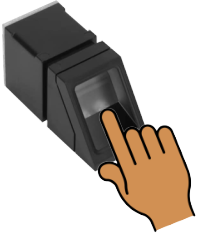
\includegraphics[scale=0.25]{fp-finger-in.png}};
    \draw[->] ($(pic cs:colok) +(-10ex,-4.5em)$) to[out=0,in=225] ($(pic cs:colok) +(0.5ex,0em)$);
    \node[anchor=east] at ($(pic cs:colok) +(-10ex,-4.5em)$) {Collection Success};
    \draw[->] ($(pic cs:col) +(-10ex,-6.5em)$) to[out=0,in=225] ($(pic cs:col) +(0.5ex,0em)$);
    \node[anchor=east] at ($(pic cs:col) +(-10ex,-6.5em)$) {Collection Step};
    \draw[->] ($(pic cs:res) +(6ex,-6.5em)$) to[out=180,in=-90] ($(pic cs:res) +(0.5ex,0em)$);
    \node[anchor=west] at ($(pic cs:resok) +(6ex,-8.5em)$) {Verification Success};
    \draw[->] ($(pic cs:resok) +(6ex,-8.5em)$) to[out=180,in=-90] ($(pic cs:resok) +(0.5ex,0em)$);
    \node[anchor=west] at ($(pic cs:res) +(6ex,-6.5em)$) {Verification Step};
    \draw[->] ($(pic cs:resid) +(6ex,-4.5em)$) to[out=180,in=-90] ($(pic cs:resid) +(2.5ex,0em)$);
    \node[anchor=west] at ($(pic cs:resid) +(6ex,-4.5em)$) {Matches with \#1};
    \draw[->] ($(pic cs:score) +(6ex,-2.5em)$) to[out=180,in=-90] ($(pic cs:score) +(2.5ex,0em)$);
    \node[anchor=west] at ($(pic cs:score) +(6ex,-2.5em)$) {Score: 68};
  \end{tikzpicture}
\end{frame}

\begin{frame}
  \frametitle{JM-101 operation details: enroll (I)}

  \begin{itemize}
    \item Enrollment sequence is triggered by
          \textbf{\texttt{PS\_AutoEnroll}} command (31H)
    \item \textbf{Input} parameters are:
  \end{itemize}

  \begin{table}
    \centering
    \footnotesize
    \begin{tabular}{ccc}
      \toprule
      ID number & \# Readings & Configuration \\
      \midrule
      2b        & 1b          & 2b            \\
      \bottomrule
    \end{tabular}
  \end{table}

  \begin{itemize}
    \item Chosen ID must be \textbf{empty} in the database
    \item Sensor sends \textbf{a minimum of 7 responses}: acknowledge,
          acquisition, generation, finger away, merge, register and result
    \item \textbf{Response} parameters are:
  \end{itemize}

  \begin{table}
    \centering
    \footnotesize
    \begin{tabular}{cc}
      \toprule
      Enrollment Step & Acquisition count/details \\
      \midrule
      1b              & 1b                        \\
      \bottomrule
    \end{tabular}
  \end{table}
\end{frame}

\begin{frame}[fragile]
  \frametitle{JM-101 operation details: enroll (II)}

  \vspace{3.5em}

  \begin{listing}[H]
    \begin{minted}[fontsize=\scriptsize,escapeinside=??]{text}
      MCU |----------------------------------------------------| SENSOR
       -> | ef 01 ff ff ff ff 01 00 08 ?\tikzmark{autoenroll}?31 ?\tikzmark{enrollid}?00 01 ?\tikzmark{readings}?02 00 00 00 3d |
          | ef 01 ff ff ff ff 07 00 05 00 00 00 00 0c          | <-
          | ef 01 ff ff ff ff 07 00 05 00 01 01 00 0e          | <-?\tikzmark{fpin1}?
          | ef 01 ff ff ff ff 07 00 05 00 02 01 00 0f          | <-
          | ef 01 ff ff ff ff 07 00 05 00 03 01 00 10          | <-?\tikzmark{fpout1}?
          | ef 01 ff ff ff ff 07 00 05 00 01 02 00 0f          | <-?\tikzmark{fpin2}?
          | ef 01 ff ff ff ff 07 00 05 00 02 02 00 10          | <-
          | ef 01 ff ff ff ff 07 00 05 00 04 f0 01 00          | <-
          | ef 01 ff ff ff ff 07 00 05 00 05 f1 01 02          | <-
          | ef 01 ff ff ff ff 07 00 05 ?\tikzmark{storeok}?00 ?\tikzmark{store}?06 f2 01 04          | <-
    \end{minted}
    \caption{\texttt{PS\_AutoEnroll} example sequence}
  \end{listing}

  \begin{tikzpicture}[overlay,remember picture]
    \draw[->] ($(pic cs:autoenroll) +(-3ex,3em)$) to[out=0,in=90] ($(pic cs:autoenroll) +(0.5ex,0.5em)$);
    \node[anchor=east] at ($(pic cs:autoenroll) +(-3ex,3em)$) {\texttt{PS\_AutoEnroll}};
    \draw[->] ($(pic cs:enrollid) +(-3ex,4.5em)$) to[out=0,in=90] ($(pic cs:enrollid) +(2.5ex,0.5em)$);
    \node[anchor=east] at ($(pic cs:enrollid) +(-3ex,4.5em)$) {Store to \#1};
    \draw[->] ($(pic cs:readings) +(-4ex,6em)$) to[out=0,in=90] ($(pic cs:readings) +(0.5ex,0.5em)$);
    \node[anchor=east] at ($(pic cs:readings) +(-4ex,6em)$) {2 readings};
    \draw[->] ($(pic cs:fpin1) +(-8ex,4.5em)$) to[out=0,in=0] (pic cs:fpin1);
    \draw[->] ($(pic cs:fpin1) +(-8ex,4.5em)$) to[out=0,in=0] (pic cs:fpin2);
    \node[anchor=east] at ($(pic cs:fpin1) +(-8ex,4.5em)$) {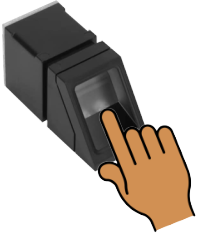
\includegraphics[scale=0.15]{fp-finger-in.png}};
    \draw[->] ($(pic cs:fpout1) +(0ex,8em)$) to[out=0,in=0] (pic cs:fpout1);
    \node[anchor=east] at ($(pic cs:fpout1) +(0ex,8em)$) {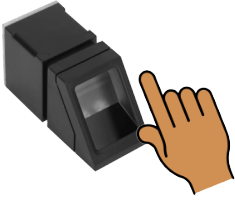
\includegraphics[scale=0.15]{fp-finger-out.png}};
    \draw[->] ($(pic cs:storeok) +(-10ex,-3.5em)$) to[out=0,in=225] ($(pic cs:storeok) +(0.5ex,0em)$);
    \node[anchor=east] at ($(pic cs:storeok) +(-10ex,-3.5em)$) {Store Success};
    \draw[->] ($(pic cs:store) +(-10ex,-5em)$) to[out=0,in=225] ($(pic cs:store) +(0.5ex,0em)$);
    \node[anchor=east] at ($(pic cs:store) +(-10ex,-5em)$) {Store Step};
  \end{tikzpicture}
\end{frame}

\begin{frame}
  \frametitle{JM-101 operation details: touch}

  \begin{itemize}
    \item When fingerprint sensor is \textbf{touched}, \texttt{TCH} output
          goes \textbf{high}
    \item Can be used to \textbf{trigger} a fingerprint verification sequence
    \item Touch sensor has a \textbf{standalone circuitry}, powered by
          \texttt{VA} pin
  \end{itemize}

  \begin{figure}
    \centering
    \begin{tikzpicture}
      \node [draw,
        minimum height=4em,
        minimum width=4em,
      ] (mcu) {MCU};
      \node [
        right=100px of mcu,
      ] (fpsensor) {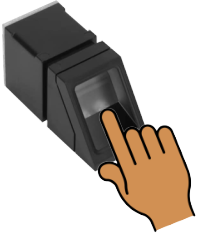
\includegraphics[scale=0.2]{fp-finger-in.png}};

      \draw[->] (fpsensor.west) -- node[above] {TCH} ++(-20px,0) -- (mcu.east);
      \draw[-,
        postaction={
            decoration={
                markings,
                mark=at position 0.5 with {\arrow{>}}
              },
            decorate
          }
      ] ($(fpsensor) +(-65px,5px)$) {} -- ++(-15px,0) -- ++(0,20px) -- ++(-15px,0);
    \end{tikzpicture}
    \caption{\texttt{TCH} output goes high when the sensor is touched}
  \end{figure}
\end{frame}

\subsection{Mapping JM-101 to the sensor API}

\begin{frame}
  \begin{center}
    \Large \textbf{Mapping JM-101 to the\\sensor API}
  \end{center}
\end{frame}

\begin{frame}
  \frametitle{The sensor driver API}

  \begin{itemize}
    \item Sensor driver API is defined in \texttt{<zephyr/drivers/sensor.h>}
    \item Provides interfaces to:
          \begin{itemize}
            \item Fetch and get sensor \textbf{data}
            \item Set and get sensor \textbf{attributes}
            \item Configure sensor \textbf{triggers}
          \end{itemize}
    \item All operations are performed on a \textbf{channel} basis
    \item \textbf{Not a perfect} fit for JM-101, but \textit{it works} if we
          abuse a little bit of the API
  \end{itemize}
\end{frame}

\begin{frame}
  \frametitle{Mapping JM-101 actions to the sensor API}

  \begin{table}
    \centering
    \footnotesize
    \begin{tabular}{ll}
      \toprule
      API call                       & JM-101 action                                    \\
      \midrule
      \texttt{sensor\_sample\_fetch} & \tabitem~Read and verify a fingerprint           \\
      \midrule
      \texttt{sensor\_channel\_get}  & \tabitem~Obtain fingerprint verification results \\
      \midrule
      \texttt{sensor\_attr\_set}     & \tabitem~Configure verification (1:1, 1:N\ldots) \\
                                     & \tabitem~Empty fingerprint database              \\
                                     & \tabitem~Trigger enrollment sequence             \\
      \midrule
      \texttt{sensor\_trigger\_set}  & \tabitem~Configure touch input interrupt         \\
      \bottomrule
    \end{tabular}
    \caption{JM-101 actions mapped to the sensor API}
  \end{table}
\end{frame}

\subsection{Coding session: JM-101 driver}

\begin{frame}
  \begin{center}
    \Large \textbf{Coding session:\\JM-101 driver}
  \end{center}
\end{frame}

\begin{frame}
  \frametitle{Coding session}

  \begin{center}
    \Huge \faInfoCircle\\
    \vspace{1ex}
    \Large \textbf{Please watch the session}\\
    \large The following slides only provide some highlights
  \end{center}
\end{frame}

\begin{frame}[fragile]
  \frametitle{File tree layout}

  \begin{listing}[H]
    \begin{minted}[fontsize=\tiny]{text}
      $ROOT: $ZEPHYR_BASE or application module root
      |-- drivers
      |   |-- CMakeLists.txt
      |   |-- Kconfig
      |   `-- sensor
      |       |-- CMakeLists.txt
      |       |-- Kconfig
      |       `-- jm101                     # Sensor driver folder
      |           |-- CMakeLists.txt        # Driver CMake file
      |           |-- Kconfig               # Driver Kconfig file
      |           `-- jm101.c               # Driver source file
      |-- dts
      |   `-- bindings
      |       `-- sensor
      |           `-- zeantec,jm101.yaml    # Devicetree bindings
      `-- include
          `-- {app|zephyr}
              `-- drivers
                  `-- sensor
                      `-- jm101.h           # Sensor custom channels,
                                            # attributes, etc.
    \end{minted}
    \caption{File tree with all relevant JM-101 sensor driver files}
  \end{listing}
\end{frame}

\begin{frame}[fragile]
  \frametitle{Devicetree bindings}

  \begin{listing}[H]
    \begin{minted}[fontsize=\tiny]{yaml}
      description: ...
      compatible: "zeantec,jm101"

      include: base.yaml

      properties:
        uart:
          type: phandle
          required: true
          description: |
            UART port to which the sensor is connected to.

        address:
          type: int
          required: false
          default: 0xffffffff
          description: |
            The address of the sensor. Defaults to 0xFFFFFFFF, which is the factory
            default.

        touch-gpios:
          type: phandle-array
          required: false
          description: |
            Touch input GPIO (active high). When the sensor is touched, the GPIO is
            set to high. It is used to trigger a fingerprint read.

    \end{minted}
    \caption{\texttt{\$ROOT/dts/bindings/sensor/zeantec,jm101.yaml}}
  \end{listing}
\end{frame}

\begin{frame}[fragile]
  \frametitle{Kconfig (I)}

  \begin{listing}[H]
    \begin{minted}[fontsize=\tiny]{kconfig}
      menu "Drivers"
      ...
      rsource "sensor/Kconfig"
      ...
      endmenu
    \end{minted}
    \caption{\texttt{\$ROOT/drivers/Kconfig}}
  \end{listing}

  \begin{listing}[H]
    \begin{minted}[fontsize=\tiny]{kconfig}
      if SENSOR
      ...
      rsource "jm101/Kconfig"
      ...
      endif # SENSOR
    \end{minted}
    \caption{\texttt{\$ROOT/drivers/sensor/Kconfig}}
  \end{listing}
\end{frame}

\begin{frame}[fragile]
  \frametitle{Kconfig (II)}

  \vspace{2.5em}

  \begin{listing}[H]
    \begin{minted}[fontsize=\tiny,escapeinside=??]{kconfig}
      DT_COMPAT_ZEANTEC_JM101 := zeantec,jm101

      config JM101
        bool "JM-101 fingerprint sensor"
        ?\tikzmark{depends}?depends on GPIO && SERIAL && UART_INTERRUPT_DRIVEN
        default $(dt_compat_enabled,$(DT_COMPAT_ZEANTEC_JM101))?\tikzmark{default}?
        help
          JM-101 fingerprint sensor.

      config JM101_TRIGGER
        bool "JM-101 touch input support"
        depends on JM101
        help
          When enabled, the JM101 can be provided with a touch input GPIO to
          trigger fingerprint readings.
    \end{minted}
    \caption{\texttt{\$ROOT/drivers/sensor/jm101/Kconfig}}
  \end{listing}

  
\begin{tikzpicture}[overlay,remember picture]
    \draw[->] ($(pic cs:depends) +(-2ex,4.7em)$) to[out=180,in=180] (pic cs:depends);
    \node[anchor=west] at ($(pic cs:depends) +(-2ex,4.7em)$) {Software Dependencies};
    \draw[->] ($(pic cs:default) +(4ex,4.5em)$) to[out=270,in=0] (pic cs:default);
    \node[anchor=south] at ($(pic cs:default) +(4ex,4.5em)$) {Enabled by default if \texttt{okay} in DT};
  \end{tikzpicture}
\end{frame}

\begin{frame}[fragile]
  \frametitle{CMake}

  \begin{listing}[H]
    \begin{minted}[fontsize=\footnotesize]{cmake}
      # include JM101 driver folder if enabled
      add_subdirectory_ifdef(CONFIG_JM101 jm101)
    \end{minted}
    \caption{\texttt{\$ROOT/drivers/sensor/CMakeLists.txt}}
  \end{listing}

  \begin{listing}[H]
    \begin{minted}[fontsize=\footnotesize]{cmake}
      # create a new Zephyr library, add sensor sources to it
      zephyr_library()
      zephyr_library_sources(jm101.c)
    \end{minted}
    \caption{\texttt{\$ROOT/drivers/sensor/jm101/CMakeLists.txt}
      \footnotemark}
  \end{listing}

  \footnotetext{Some driver classes have a single library, tipically drivers
    where a single implementation is chosen. In such cases,
    \texttt{zephyr\_library\_amend} should be used instead.}
\end{frame}

\begin{frame}[fragile]
  \frametitle{Driver highlights (I)}

  \begin{itemize}
    \item \textbf{Standard} channels/attributes are \textbf{not sufficient}
          for JM-101
    \item \textbf{Private/custom} channels are defined in a \textbf{public}
          header
  \end{itemize}

  \begin{listing}[H]
    \begin{minted}[fontsize=\tiny]{c}
      #include <zephyr/drivers/sensor.h>

      /** @brief Any identifier (used to do 1:N identification). */
      #define JM101_ID_ANY 0xFFFFU

      /** @brief JM101 custom channels. */
      enum jm101_channel {
        /** Fingerprint verification. */
        JM101_CHAN_FINGERPRINT = SENSOR_CHAN_PRIV_START,
      };

      /** @brief JM101 custom attributes. */
      enum jm101_attribute {
        /** Fingerprint ID used when verifying. */
        JM101_ATTR_ID_NUM = SENSOR_ATTR_PRIV_START,
        /** Run the enrolling sequence. */
        JM101_ATTR_ENROLL,
        /** Emtpies the fingerprint database. */
        JM101_ATTR_EMPTYDB,
      };
    \end{minted}
    \caption{\texttt{\$ROOT/include/app|zephyr/sensor/jm101.h}}
  \end{listing}
\end{frame}

\begin{frame}[fragile]
  \frametitle{Driver highlights (II)}

  \begin{listing}[H]
    \begin{minted}[fontsize=\tiny]{c}
      /* We're implementing a driver for the zeantec,jm101 compatible */
      #define DT_DRV_COMPAT zeantec_jm101
    \end{minted}
    \caption{Definition of the driver's compatible}
  \end{listing}
\end{frame}

\begin{frame}[fragile]
  \frametitle{Driver highlights (III)}

  \begin{listing}[H]
    \begin{minted}[fontsize=\tiny]{c}
      /* We need to define a device: DEVICE_DT_INST_DEFINE */
      #include <zephyr/device.h>
      /* We need to retrieve information from Devicetree */
      #include <zephyr/devicetree.h>
      /* We need to control the TOUCH input GPIO */
      #include <zephyr/drivers/gpio.h>
      /* We need to define the sensor API ops */
      #include <zephyr/drivers/sensor.h>
      /* We communicate with the sensor via UART */
      #include <zephyr/drivers/uart.h>
      /* Adding some logging is always useful */
      #include <zephyr/logging/log.h>
      /* We'll be manipulating big-endian data */
      #include <zephyr/sys/byteorder.h>
      /* We'll need utilities like IF_ENABLED */
      #include <zephyr/sys/util_macro.h>

      /* We have custom channels/attributes */
      #include <app/drivers/sensor/jm101.h>
    \end{minted}
    \caption{All required includes for the JM-101 driver}
  \end{listing}
\end{frame}

\begin{frame}[fragile]
  \frametitle{Driver highlights (IV)}

  \begin{itemize}
    \item Driver is made \textbf{multi-instance} by combining both
          \texttt{DT\_INST\_FOREACH\_STATUS\_OKAY} and \texttt{JM101\_DEFINE}
  \end{itemize}

  \begin{listing}[H]
    \begin{minted}[fontsize=\tiny]{c}
      #define JM101_DEFINE(i)                                                  \
        static struct jm101_data jm101_data_##i = {                            \
          .verify_id = JM101_ID_ANY,                                           \
        };                                                                     \
                                                                               \
        /* pull instance configuration from Devicetree */                      \
        static const struct jm101_config jm101_config_##i = {                  \
          .uart = DEVICE_DT_GET(DT_INST_PHANDLE(i, uart)),                     \
          .addr = DT_INST_PROP(i, address),                                    \
          IF_ENABLED(CONFIG_JM101_TRIGGER,                                     \
                     (.touch = GPIO_DT_SPEC_INST_GET_OR(i, touch_gpios, {}), ))\
        };                                                                     \
                                                                               \
        /* define a new device inst. with the data and config defined above */ \
        DEVICE_DT_INST_DEFINE(i, jm101_init, NULL, &jm101_data_##i,            \
                              &jm101_config_##i, POST_KERNEL,                  \
                              CONFIG_SENSOR_INIT_PRIORITY, &jm101_api);

      /* expand JM101_DEFINE for all instances defined in Devicetree with
       * status "okay"
       */
      DT_INST_FOREACH_STATUS_OKAY(JM101_DEFINE)
    \end{minted}
    \caption{JM-101 instantiation}
  \end{listing}
\end{frame}

\begin{frame}[fragile]
  \frametitle{Driver highlights (V)}

  \begin{itemize}
    \item All other devices used by the driver must be
          \textbf{checked for readiness} when driver is initialized
  \end{itemize}

  \begin{listing}[H]
    \begin{minted}[fontsize=\tiny]{c}
      static int jm101_init(const struct device *dev)
      {
        const struct jm101_config *config = dev->config;
        ...

        if (!device_is_ready(config->uart)) {
          LOG_ERR("UART not ready");
          return -ENODEV;
        }

        ...
      #ifdef CONFIG_JM101_TRIGGER
        if (config->touch.port != NULL) {
          if (!device_is_ready(config->touch.port)) {
            LOG_ERR("Touch GPIO controller not ready");
            return -ENODEV;
          }
          ...
      #endif
        ...
      }
    \end{minted}
    \caption{JM-101 instantiation}
  \end{listing}
\end{frame}

\begin{frame}[fragile]
  \frametitle{Driver highlights (VI)}

  \begin{itemize}
    \item A message queue (\mintinline{c}{struct k_msgq}) is used to store
          received packets
    \item Allows CPU to \textbf{idle} while waiting for sensor to respond
  \end{itemize}

  \begin{listing}[H]
    \begin{minted}[fontsize=\tiny]{c}
      static void uart_cb_rx_handler(const struct device *dev)
      {
        ...
        if (data->buf_ctr >= PKT_LEN(data->rx_data_len)) {
          k_msgq_put(&data->rx_queue, data->buf, K_NO_WAIT);
          ...
        }
      }

      static int jm101_recv(const struct device *dev, uint8_t *result,
                            uint8_t *rx_data, uint8_t rx_data_len)
      {
        ...
        ret = k_msgq_get(&data->rx_queue, buf, RX_TIMEOUT);
        ...
      }
    \end{minted}
    \caption{Usage of message queues to receive packets}
  \end{listing}
\end{frame}

\subsection{Using the JM-101 driver}

\begin{frame}
  \begin{center}
    \Large \textbf{Using the\\JM-101 Driver}
  \end{center}
\end{frame}

\begin{frame}[fragile]
  \frametitle{Devicetree device definition}

  \begin{listing}[H]
    \begin{minted}[fontsize=\tiny]{dts}
      / {
          fpreader: jm101 {
              compatible = "zeantec,jm101";
              label = "JM101";
              uart = <&uart1>;
              touch-gpios = <&gpio1 4 GPIO_ACTIVE_HIGH>;
          };
      };
    \end{minted}
    \caption{Devicetree definition of one JM-101 device instance}
  \end{listing}
\end{frame}

\begin{frame}[fragile]
  \frametitle{Project configuration}

  \begin{itemize}
    \item JM-101 sensor driver is enabled when \texttt{CONFIG\_JM101=y}
    \item \texttt{CONFIG\_JM101} is automatically enabled if:
          \begin{itemize}
            \item All its \textbf{dependencies} are \textbf{enabled}, including
                  \texttt{CONFIG\_SENSOR}
            \item One or more instances are \texttt{okay} in Devicetree
          \end{itemize}
  \end{itemize}
  \begin{listing}[H]
    \begin{minted}[fontsize=\tiny]{kconfig}
      # dependencies required so that JM-101 driver can be enabled
      CONFIG_GPIO=y
      CONFIG_SERIAL=y
      CONFIG_UART_INTERRUPT_DRIVEN=y

      # enable the sensor driver class
      CONFIG_SENSOR=y

      # Optional, only if we need trigger support
      CONFIG_JM101_TRIGGER=y
    \end{minted}
    \caption{Project configuration (\texttt{prj.conf})}
  \end{listing}
\end{frame}

\begin{frame}[fragile]
  \frametitle{Obtain a reference to a device instance}

  \begin{listing}[H]
    \begin{minted}[fontsize=\tiny]{c}
      /* reference resolved at compile time (using unique node label) */
      const struct device *fpreader = DEVICE_DT_GET(DT_NODELABEL(fpreader));

      /* verify for device readiness before operation */
      if (!device_is_ready(fpreader)) {
          printk("Fingerprint sensor device not ready\n");
          return -ENODEV;
      }
    \end{minted}
    \caption{Obtain a reference to the \texttt{fpreader} device and verify
      if ready}
  \end{listing}
\end{frame}

\begin{frame}[fragile]
  \frametitle{Example: verify a fingerprint}

  \begin{listing}[H]
    \begin{minted}[fontsize=\tiny]{c}
      /* configure verification (optional) */
      struct sensor_value val = {
        .val1 = JM101_ID_ANY, /* 1:N verification */
      };

      sensor_attr_set(fpreader, JM101_CHAN_FINGERPRINT,
                      JM101_ATTR_ID_NUM, &val);

      /* start fingerprint verification */
      ret = sensor_sample_fetch_chan(dev, JM101_CHAN_FINGERPRINT);
      if (ret < 0) {
        printk("Verification failed\n");
        return ret;
      }

      /* obtain verification results */
      sensor_channel_get(dev, JM101_CHAN_FINGERPRINT, &val);

      printk("Verified fingerprint #%d, score: %d\n", val.val1, val.val2);
    \end{minted}
    \caption{Example code to verify a fingerprint}
  \end{listing}
\end{frame}

\begin{frame}[fragile]
  \frametitle{Example: register a fingerprint}

  \begin{listing}[H]
    \begin{minted}[fontsize=\tiny]{c}
      /* empty database first (optional) */
      ret = sensor_attr_set(fpreader, JM101_CHAN_FINGERPRINT,
                            JM101_ATTR_EMPTYDB, NULL);
      if (ret < 0) {
        printk("Failed to empty database\n");
        return ret;
      }

      /* enroll */
      struct sensor_value val = {
        .val1 = 1U, /* store as fingerprint ID #1 */
        .val2 = 2U, /* number of readings */
      };

      ret = sensor_attr_set(fpreader, JM101_CHAN_FINGERPRINT,
                            JM101_ATTR_ENROLL, &val);
      if (ret < 0) {
        printk("Failed to enroll\n");
        return ret;
      }

      printk("Enrollment finished\n");
    \end{minted}
    \caption{Example code to register a fingerprint}
  \end{listing}
\end{frame}

\begin{frame}[fragile]
  \frametitle{Example: configure trigger}

  \begin{listing}[H]
    \begin{minted}[fontsize=\tiny]{c}
      void fp_trig_handler(const struct device *dev,
                           const struct sensor_trigger *trigger)
      {
        /* perform here a fingerprint verification */
      }
      
      const struct sensor_trigger trig = {
        .type = SENSOR_TRIG_TAP,
        .chan = JM101_CHAN_FINGERPRINT,
      };
      
      /* configure fingerprint trigger */
      ret = sensor_trigger_set(fpreader, &trig, fp_trig_handler);
      if (ret < 0) {
        printk("Failed to configure trigger\n");
        return ret;
      }
    \end{minted}
    \caption{Example code to configure touch trigger}
  \end{listing}
\end{frame}

% section: going custom --------------------------------------------------------

\section{Going custom}

\begin{frame}
  \begin{center}
    \Huge \textbf{Going custom}
  \end{center}
\end{frame}

\subsection{Motivation}

\begin{frame}
  \begin{center}
    \Large \textbf{Motivation}
  \end{center}
\end{frame}

\begin{frame}
  \frametitle{Why creating a custom API?}

  \begin{itemize}
    \item \textbf{Upstream} APIs tend to be designed for \textbf{common}
          peripherals, e.g.\ I2C, SPI, GPIO\ldots
    \item MCUs often have highly \textbf{specialized} peripherals,
          \textbf{difficult} to integrate into a vendor \textbf{generic} API
    \item Such peripherals are frequently used in \textbf{specific domains},
          e.g.\ power electronics, BMS, etc.
    \item Applications may have a \textbf{wide range of requirements}:
          difficult to create generic APIs that fit all usecases
    \item \textbf{Upstream} APIs often do \textbf{not} solve complex usecases
          nor use all hardware features (e.g.\ ADC)
  \end{itemize}
\end{frame}

\subsection{An API to control locks}

\begin{frame}
  \begin{center}
    \Large \textbf{An API to control locks}
  \end{center}
\end{frame}

\begin{frame}
  \frametitle{Lock API design}

  \begin{itemize}
    \item The lock API has the following requirements:
          \begin{itemize}
            \item Ability to \textbf{open} and \textbf{close} the lock
            \item Operations succeed only if the action is \textbf{completed}
          \end{itemize}
    \item \textbf{Multiple} drivers can be implemented:
          \begin{itemize}
            \item Lock driven by a servo with feedback
            \item Lock driven by a DC motor with feedback
            \item Lock driven by a DC motor with inductive position sensors
            \item \ldots
          \end{itemize}
    \item A \textbf{fake/mock} device can also be implemented for
          \textbf{testing}
  \end{itemize}
\end{frame}

\begin{frame}[fragile]
  \frametitle{File Tree Layout}

  \begin{listing}[H]
    \begin{minted}[fontsize=\tiny]{text}
      $ROOT: application module root
      |-- drivers
      |       |-- CMakeLists.txt
      |       |-- Kconfig
      |       `-- lock                      # Lock drivers folder
      |           |-- CMakeLists.txt        # Lock drivers CMake file
      |           |-- Kconfig               # Lock drivers Kconfig file
      |           |-- Kconfig.vnd_dev       # Kconfig for vnd,dev
      |           `-- vnd_dev.c             # Driver for vnd,dev
      |-- dts
      |   `-- bindings
      |       `-- lock
      |           `-- vnd,dev.yaml          # Devicetree bindings for vnd,dev
      `-- include
          `-- app
              `-- drivers
                  `-- lock.h                # Public header with the lock API
    \end{minted}
    \caption{File tree with all relevant lock API files}
  \end{listing}
\end{frame}

\begin{frame}[fragile]
  \frametitle{Lock API driver ops}

  \begin{listing}[H]
    \begin{minted}[fontsize=\tiny]{c}
      typedef int (*lock_open_t)(const struct device *dev);
      typedef int (*lock_close_t)(const struct device *dev);

      __subsystem struct lock_driver_api {
        lock_open_t open;
        lock_close_t close;
      };
    \end{minted}
    \caption{Lock API driver ops, \texttt{\$ROOT/include/app/drivers/lock.h}}
  \end{listing}
\end{frame}

\begin{frame}[fragile]
  \frametitle{Lock API interface (I)}

  \begin{listing}[H]
    \begin{minted}[fontsize=\tiny]{c}
      /**
      * @brief Open the lock.
      *
      * @param dev Lock device instance.
      *
      * @retval 0 On success.
      * @retval -errno Other negative errno in case of failure.
      */
      __syscall int lock_open(const struct device *dev);
  
      static inline int z_impl_lock_open(const struct device *dev)
      {
        const struct lock_driver_api *api =
          (const struct lock_driver_api *)dev->api;

        return api->open(dev);
      }
      ...
    \end{minted}
    \caption{Lock API interface,
      \texttt{\$ROOT/include/app/drivers/lock.h}}
  \end{listing}
\end{frame}

\begin{frame}[fragile]
  \frametitle{Lock API interface (II)}

  \begin{listing}[H]
    \begin{minted}[fontsize=\tiny]{c}
      ...
      /**
      * @brief Close the lock.
      *
      * @param dev Lock device instance.
      *
      * @retval 0 On success.
      * @retval -errno Other negative errno in case of failure.
      */
      __syscall int lock_close(const struct device *dev);

      static inline int z_impl_lock_close(const struct device *dev)
      {
        const struct lock_driver_api *api =
          (const struct lock_driver_api *)dev->api;

        return api->close(dev);
      }

      #include <syscalls/lock.h>
    \end{minted}
    \caption{Lock API interface,
      \texttt{\$ROOT/include/app/drivers/lock.h}}
  \end{listing}
\end{frame}

\begin{frame}[fragile]
  \frametitle{A note about userspace}

  \begin{itemize}
    \item Even if optional, adding support \textbf{userspace} increases
          \textbf{complexity}
    \item Sometimes an application may \textbf{never need userspace} support
    \item Some APIs may always be used in \textbf{Kernel space}
  \end{itemize}

  \begin{listing}[H]
    \begin{minted}[fontsize=\tiny]{c}
      /**
      * @brief Open the lock (no userspace support).
      *
      * @param dev Lock device instance.
      *
      * @retval 0 On success.
      * @retval -errno Other negative errno in case of failure.
      */
      static inline int lock_open(const struct device *dev)
      {
        const struct lock_driver_api *api =
          (const struct lock_driver_api *)dev->api;

        return api->open(dev);
      }
    \end{minted}
    \caption{Lock API interface without userspace support}
  \end{listing}
\end{frame}

\subsection{A servo driven lock}

\begin{frame}
  \begin{center}
    \Large \textbf{A servo-driven lock}
  \end{center}
\end{frame}

\begin{frame}
  \frametitle{A servo-driven lock}

  \begin{itemize}
    \item<-1> A \textbf{PWM controlled servo} controls the \textbf{position} of
          the lock: open or closed
    \item The servo provides \textbf{position feedback} as an \textbf{analog}
          signal proportional to its position
  \end{itemize}

  \begin{figure}
    \centering
    \begin{columns}
      \begin{column}{0.5\textwidth}
        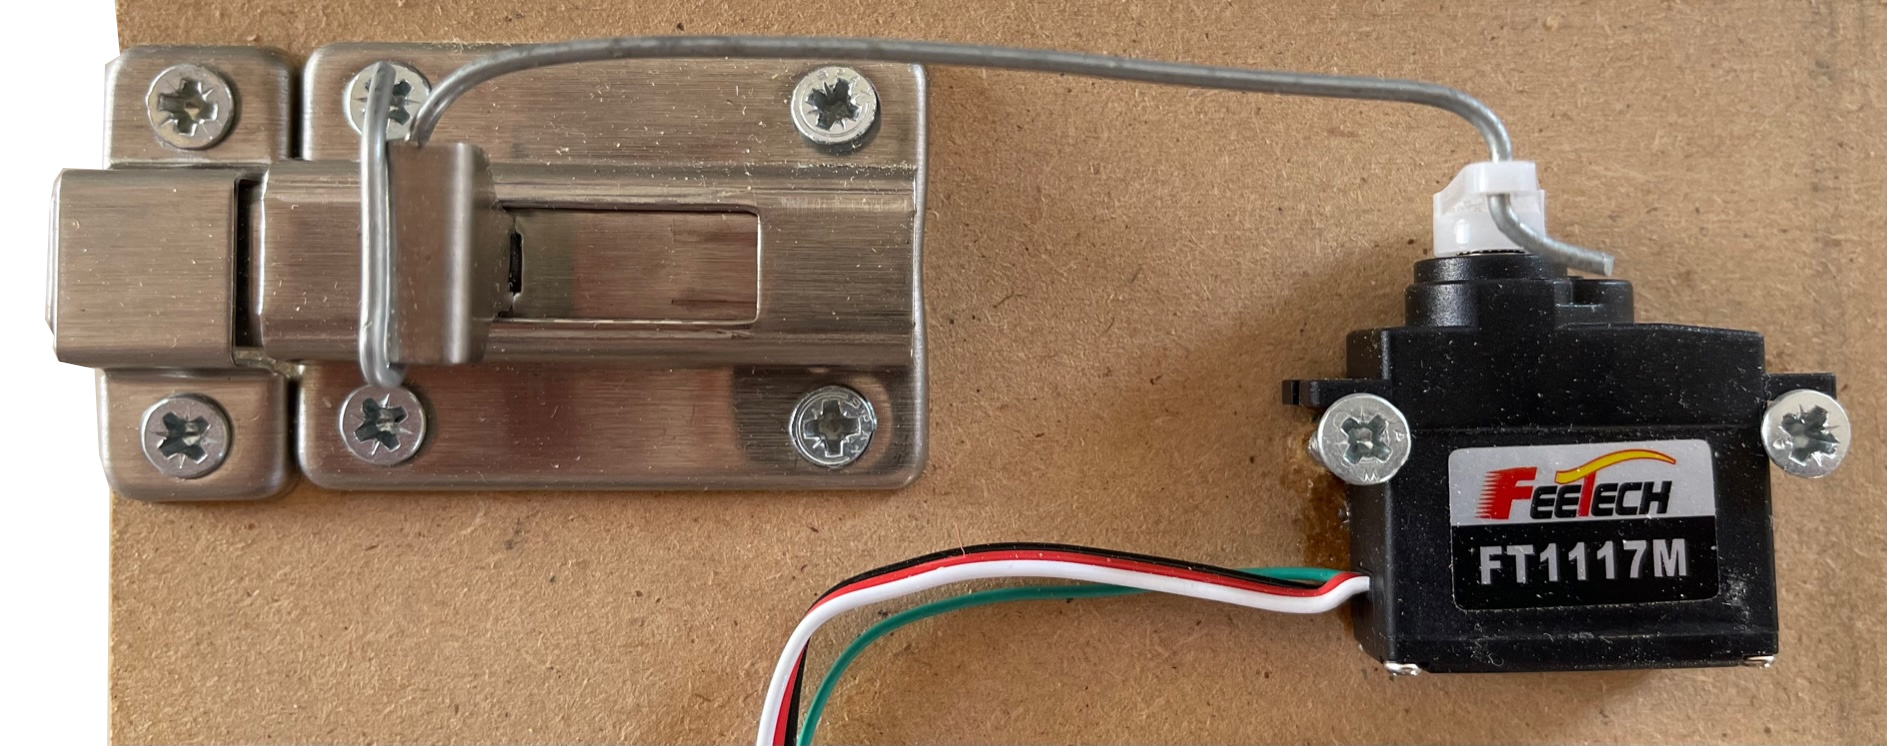
\includegraphics[width=\textwidth]{lock-closed.jpg}
      \end{column}
      \begin{column}{0.5\textwidth}
        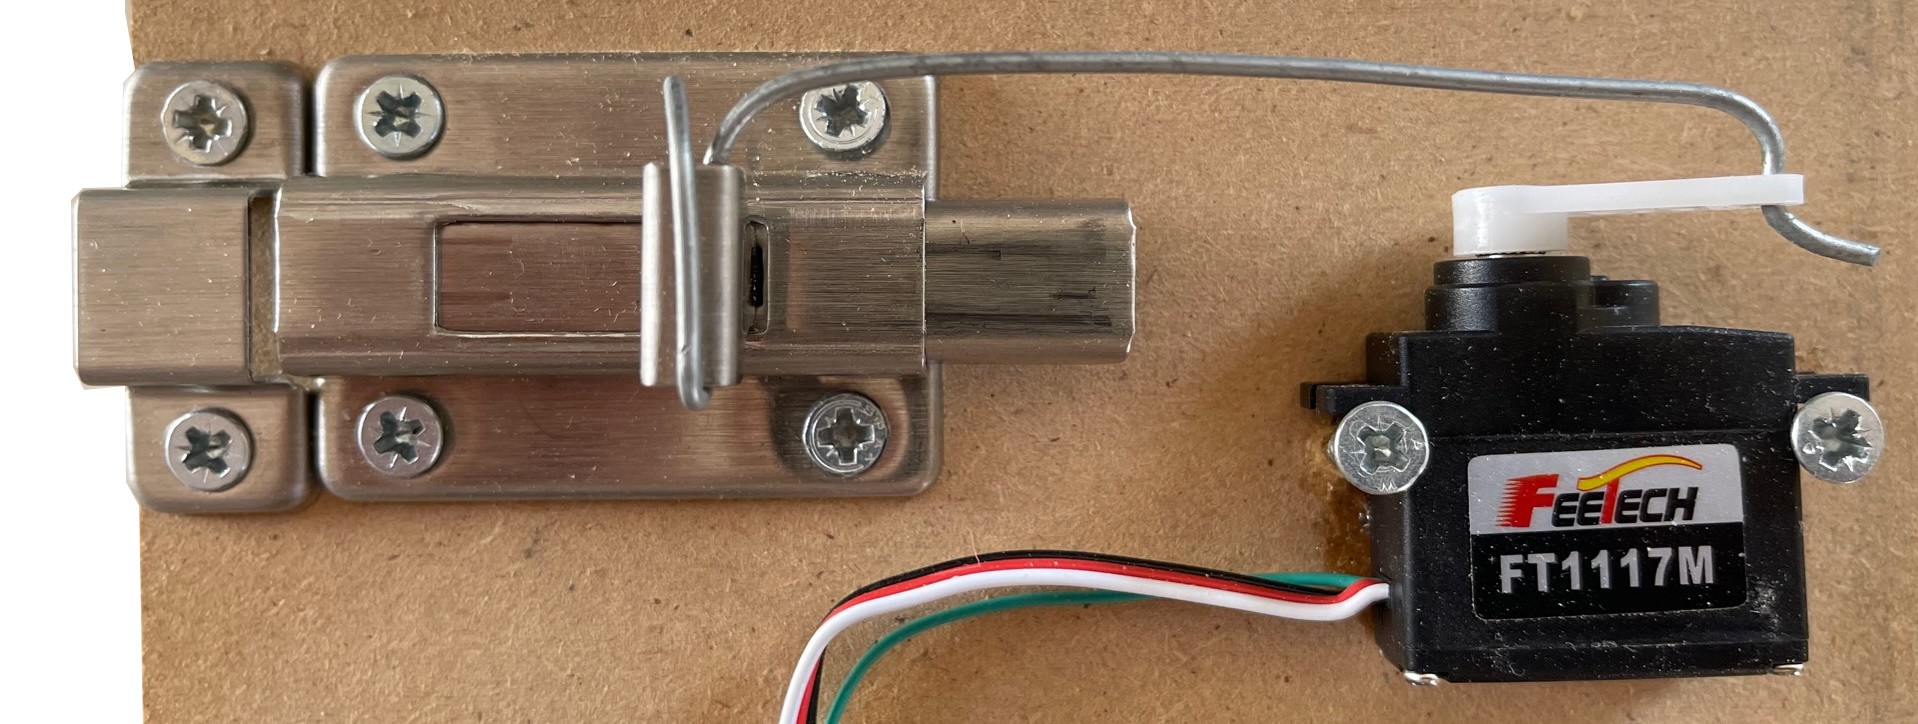
\includegraphics[width=\textwidth]{lock-open.jpg}
      \end{column}
    \end{columns}
    \caption{Servo-driven lock, closed (left) and open (right)}
  \end{figure}
\end{frame}

\begin{frame}
  \frametitle{Servo Positioning}

  \begin{itemize}
    \item<-1> Servos are tipically controlled by a \textbf{PWM} signal, making
          their \textbf{position $\theta$ proportional} to the
          \textbf{pulse width $w$}
  \end{itemize}

  \begin{figure}
    \centering
    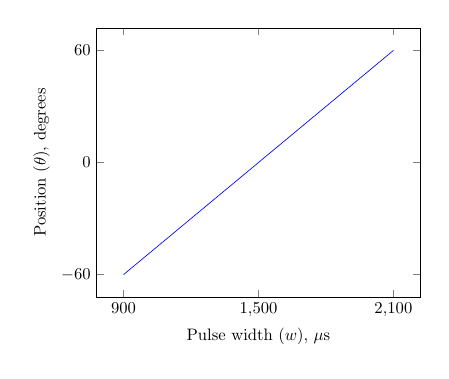
\begin{tikzpicture}[scale=0.6]
      \begin{axis}[
          xlabel = {Pulse width ($w$), $\mu\mathrm{s}$},
          ylabel = {Position ($\theta$), degrees},
          xtick = {900, 1500, 2100},
          ytick = {-60, 0, 60},
        ]
        \addplot [
          domain=900:2100,
          samples=3,
          color=blue,
        ]
        {0.1*x - 150};
      \end{axis}
    \end{tikzpicture}
    \caption{Position vs.\ pulse width for the FT1117M servo}
  \end{figure}
\end{frame}

\begin{frame}
  \frametitle{Servo Analog Feedback}

  \begin{itemize}
    \item<-1> The voltage $v$ given by the analog feedback is proportional to
          servo's current position $\theta$, by a gain factor $G$ with an added
          offset $K$:
  \end{itemize}
  \[
    v = G\theta + K
  \]
  \begin{itemize}
    \item<-2> For convenience, and because position is proportional to the pulse
          width, it can also be written as a function of the
          pulse width:
  \end{itemize}
  \[
    v = G'w + K
  \]

  \begin{table}
    \centering
    \begin{tabular}{cc}
      \toprule
      Gain                                       & Offset                 \\
      \midrule
      $-1.765~\frac{\textrm{mV}}{\mu\textrm{s}}$ & $4206.250~\textrm{mV}$ \\
      \bottomrule
    \end{tabular}
    \caption{Gain and offset for the FT1117M servo}
  \end{table}
\end{frame}

\subsection{Coding session: servo-driven lock}

\begin{frame}
  \begin{center}
    \Large \textbf{Coding session: servo-driven lock}
  \end{center}
\end{frame}

\begin{frame}
  \frametitle{Coding session}

  \begin{center}
    \Huge \faInfoCircle\\
    \vspace{1ex}
    \Large \textbf{Please watch the session}\\
    \large The following slides only provide some highlights
  \end{center}
\end{frame}

\begin{frame}[fragile]
  \frametitle{File Tree Layout}

  \begin{listing}[H]
    \begin{minted}[fontsize=\tiny]{text}
      $ROOT: application module root
      |-- CMakeLists.txt
      |-- drivers
      |       |-- CMakeLists.txt
      |       `-- lock                      # Lock drivers folder
      |           |-- CMakeLists.txt        # Lock drivers CMake file
      |           |-- Kconfig               # Lock drivers Kconfig file
      |           |-- Kconfig.servo         # Kconfig for lock-servo
      |           `-- servo.c               # Driver for lock-servo
      `-- dts
          `-- bindings
              `-- lock
                  `-- lock-servo.yaml       # Devicetree bindings for lock-servo
    \end{minted}
    \caption{File tree with all relevant files for the servo-driven lock driver}
  \end{listing}
\end{frame}

\begin{frame}[fragile]
  \frametitle{Devicetree bindings (I)}

  \begin{listing}[H]
    \begin{minted}[fontsize=\tiny]{yaml}
      description: Lock driven by a servo

      compatible: "lock-servo"

      include: base.yaml

      properties:
          pwms:
            required: true
            type: phandle-array
            description: |
              PWM specifier driving the servo motor.

          open-pulse-us:
            required: true
            type: int
            description: |
              Lock open position pulse width (microseconds).

          closed-pulse-us:
            required: true
            type: int
            description: |
              Lock closed position pulse width (microseconds).
          ...
    \end{minted}
    \caption{\texttt{\$ROOT/dts/bindings/lock/lock-servo.yaml}}
  \end{listing}
\end{frame}

\begin{frame}[fragile]
  \frametitle{Devicetree bindings (II)}

  \begin{listing}[H]
    \begin{minted}[fontsize=\tiny]{yaml}
          ...
          io-channels:
            required: true
            type: phandle-array
            description: |
              ADC specifier for servo feedback.

          fb-gain:
            required: true
            type: int
            description: |
              Servo feedback gain (uV/usec).

          fb-offset:
            required: true
            type: int
            description: |
              Servo feedback offset (uV).
          ...
    \end{minted}
    \caption{\texttt{\$ROOT/dts/bindings/lock/lock-servo.yaml}}
  \end{listing}
\end{frame}

\begin{frame}[fragile]
  \frametitle{Devicetree bindings (III)}

  \begin{listing}[H]
    \begin{minted}[fontsize=\tiny]{yaml}
          ...
          max-target-err-us:
            required: true
            type: int
            description: |
              Maximum target pulse error (+/-), in microseconds.

          max-action-time-ms:
            required: true
            type: int
            description: |
              Maximum time to complete open/close actions (msec).
    \end{minted}
    \caption{\texttt{\$ROOT/dts/bindings/lock/lock-servo.yaml}}
  \end{listing}
\end{frame}

\begin{frame}[fragile]
  \frametitle{Kconfig (I)}

  \begin{listing}[H]
    \begin{minted}[fontsize=\tiny]{kconfig}
      menu "Drivers"
      ...
      rsource "lock/Kconfig"
      ...
      endmenu
    \end{minted}
    \caption{\texttt{\$ROOT/drivers/Kconfig}}
  \end{listing}
\end{frame}

\begin{frame}[fragile]
  \frametitle{Kconfig (II)}
  \begin{listing}[H]
    \begin{minted}[fontsize=\tiny]{kconfig}
      menuconfig LOCK
      bool "Locks"
    
      if LOCK

      # define lock logging module
      module = LOCK
      module-str = lock
      source "subsys/logging/Kconfig.template.log_config"

      # define lock drivers init priority
      config LOCK_INIT_PRIORITY
        int "Lock init priority"
        default 90
        help
          Lock initialization priority.

      # include each implementation's Kconfig
      rsource "Kconfig.servo"

      endif # LOCK
    \end{minted}
    \caption{\texttt{\$ROOT/drivers/lock/Kconfig}}
  \end{listing}
\end{frame}

\begin{frame}[fragile]
  \frametitle{Kconfig (III)}
  \begin{listing}[H]
    \begin{minted}[fontsize=\tiny]{kconfig}
      DT_COMPAT_LOCK_SERVO := lock-servo

      config LOCK_SERVO
        bool "Servo-controlled lock"
        depends on PWM && ADC
        default $(dt_compat_enabled,$(DT_COMPAT_LOCK_SERVO))
        help
          Enables a servo-controlled lock driver.

    \end{minted}
    \caption{\texttt{\$ROOT/drivers/lock/Kconfig.servo}}
  \end{listing}
\end{frame}

\begin{frame}[fragile]
  \frametitle{CMake}

  \begin{listing}[H]
    \begin{minted}[fontsize=\tiny]{cmake}
      add_subdirectory(drivers)

      zephyr_include_directories(include)

      # optional, only needed for userspace support
      list(APPEND SYSCALL_INCLUDE_DIRS ${CMAKE_CURRENT_SOURCE_DIR}/include)
      set(SYSCALL_INCLUDE_DIRS ${SYSCALL_INCLUDE_DIRS} PARENT_SCOPE)
    \end{minted}
    \caption{\texttt{\$ROOT/CMakeLists.txt}}
  \end{listing}

  \begin{listing}[H]
    \begin{minted}[fontsize=\tiny]{cmake}
      add_subdirectory_ifdef(CONFIG_LOCK lock)
    \end{minted}
    \caption{\texttt{\$ROOT/drivers/CMakeLists.txt}}
  \end{listing}

  \begin{listing}[H]
    \begin{minted}[fontsize=\tiny]{cmake}
      zephyr_library()
      zephyr_library_sources_ifdef(CONFIG_LOCK_SERVO servo.c)
    \end{minted}
    \caption{\texttt{\$ROOT/drivers/lock/CMakeLists.txt}}
  \end{listing}
\end{frame}

\begin{frame}[fragile]
  \frametitle{Driver highlights (I)}

  \begin{itemize}
    \item Driver makes use of the PWM API \textbf{DT-spec} facilities
    \item Allows to \textbf{easily collect} all PWM property cells from DT
    \item Makes code \textbf{less verbose}
  \end{itemize}

  \begin{listing}[H]
    \begin{minted}[fontsize=\tiny]{c}
        struct lock_servo_config {
          ...
          /* PWM specifier for servo motor */
          struct pwm_dt_spec servo;
          ...
        };

        /* using *_dt APIs makes code less verbose */
        ret = pwm_set_pulse_dt(&config->servo, target_pulse);
        ...

        /* PWM specifier is initialized using PWM_DT_INST_SPEC_GET() */
        #define LOCK_SERVO_DEFINE(i)                                           \
          static const struct lock_servo_config lock_servo_config_##i = {      \
            .servo = PWM_DT_INST_SPEC_GET(i),                                  \
            ...
    \end{minted}
    \caption{Usage of PWM DT-spec facilities within the servo lock driver}
  \end{listing}
\end{frame}

\begin{frame}[fragile]
  \frametitle{Driver highlights (II)}

  \begin{itemize}
    \item Driver makes use of the ADC API \textbf{DT-spec} facilities
    \item Allows to \textbf{easily collect} all ADC configuration from DT
  \end{itemize}

  \begin{listing}[H]
    \begin{minted}[fontsize=\tiny]{c}
        struct lock_servo_config {
          ...
          /* ADC specifier for servo feedback */
          struct adc_dt_spec adc;
          ...
        };

        /* ADC specifier is initialized using ADC_DT_INST_SPEC_GET() */
        #define LOCK_SERVO_DEFINE(i)                                           \
          static const struct lock_servo_config lock_servo_config_##i = {      \
            .adc = ADC_DT_INST_SPEC_GET(i),                                    \
            ...
    \end{minted}
    \caption{Usage of ADC DT-spec facilities within the servo lock driver}
  \end{listing}
\end{frame}

\subsection{Using the servo-driven lock driver}

\begin{frame}
  \begin{center}
    \Large \textbf{Using the servo-driven\\lock driver}
  \end{center}
\end{frame}

\begin{frame}[fragile]
  \frametitle{Devicetree Definition}

  \begin{listing}[H]
    \begin{minted}[fontsize=\tiny]{dts}
      / {
        lock: lock-servo {
          compatible = "lock-servo";
          pwms = <&pwm0 0 PWM_MSEC(20) PWM_POLARITY_NORMAL>;
          open-pulse-us = <2100>;
          closed-pulse-us = <1250>;
          io-channels = <&adc 0>;
          fb-gain = <(-1765)>;
          fb-offset = <4206250>;
          max-target-err-us = <50>;
          max-action-time-ms = <2000>;
        };
      };
    \end{minted}
    \caption{Devicetree definition of one servo-driven lock device instance}
  \end{listing}
\end{frame}

\begin{frame}[fragile]
  \frametitle{Configuration of the ADC in Devicetree}

  \begin{listing}[H]
    \begin{minted}[fontsize=\tiny]{dts}
      &adc {
        #address-cells = <1>;
        #size-cells = <0>;

        /* configuration suitable for servo feedback measurements
         * servo feedback range ~= (0.5V - 2.7V)
         * ADC range when using internal ref = (0.0V - 0.6V), gain <= 1/6
         */
        channel@0 {
          reg = <0>;
          zephyr,gain = "ADC_GAIN_1_6";
          zephyr,reference = "ADC_REF_INTERNAL";
          zephyr,acquisition-time = <ADC_ACQ_TIME_DEFAULT>;
          zephyr,input-positive = <NRF_SAADC_AIN1>;
          zephyr,resolution = <12>;
        };
      };
    \end{minted}
    \caption{ADC configuration specified in Devicetree (platform specific)}
  \end{listing}
\end{frame}

\begin{frame}[fragile]
  \frametitle{Pin control configuration in Devicetree}

  \begin{listing}[H]
    \begin{minted}[fontsize=\tiny]{dts}
      /* assign PWM0 channel 0 to P1.03 */
      &pwm0_default {
        group1 {
          psels = <NRF_PSEL(PWM_OUT0, 1, 3)>;
        };
      };

      &pwm0_sleep {
        group1 {
          psels = <NRF_PSEL(PWM_OUT0, 1, 3)>;
        };
      };
    \end{minted}
    \caption{PWM pinctrl overrides for nRF52840DK (platform specific)}
  \end{listing}
\end{frame}

\begin{frame}[fragile]
  \frametitle{Project Configuration}

  \begin{itemize}
    \item Servo-driven lock driver is enabled when
          \texttt{CONFIG\_LOCK\_SERVO=y}
    \item \texttt{CONFIG\_LOCK\_SERVO} is automatically enabled if:
          \begin{itemize}
            \item All its \textbf{dependencies} are \textbf{enabled}, including
                  \texttt{CONFIG\_LOCK}
            \item One or more instances are \texttt{okay} in Devicetree
          \end{itemize}
  \end{itemize}
  \begin{listing}[H]
    \begin{minted}[fontsize=\tiny]{kconfig}
      # dependencies required so that servo-driven lock driver can be enabled
      CONFIG_ADC=y
      CONFIG_PWM=y

      # enable the lock driver class
      CONFIG_LOCK=y
    \end{minted}
    \caption{Project configuration (\texttt{prj.conf})}
  \end{listing}
\end{frame}

\begin{frame}[fragile]
  \frametitle{Obtain a Reference to a Device Instance}

  \begin{listing}[H]
    \begin{minted}[fontsize=\tiny]{c}
      /* reference resolved at compile time (using unique node label) */
      const struct device *lock = DEVICE_DT_GET(DT_NODELABEL(lock));

      /* verify for device readiness before operation */
      if (!device_is_ready(lock)) {
          printk("Lock device not ready\n");
          return -ENODEV;
      }
    \end{minted}
    \caption{Obtain a reference to the \texttt{lock} device and verify if ready}
  \end{listing}
\end{frame}

\begin{frame}[fragile]
  \frametitle{Example: open and close}

  \begin{listing}[H]
    \begin{minted}[fontsize=\tiny]{c}
      ret = lock_open(lock);
      if (ret < 0) {
        printk("Could not open lock: %d\n", ret);
        return ret;
      }

      ret = lock_close(lock);
      if (ret < 0) {
        printk("Could not close lock: %d\n", ret);
        return ret;
      }
    \end{minted}
    \caption{Example code to open and close the lock}
  \end{listing}
\end{frame}

% section: conclusions ---------------------------------------------------------

\section{Conclusions}

\begin{frame}
  \begin{center}
    \Huge
    \textbf{Conclusions}
  \end{center}
\end{frame}

\begin{frame}
  \frametitle{Conclusions}

  \begin{itemize}
    \item \textbf{Devicetree} is nowadays \textbf{core} to the Zephyr device
          model
    \item Devicetree allows to easily \textbf{define N instances} of a device,
          each with its \textbf{own} configuration
    \item Devicetree does not \textbf{\textit{exist}} after compiling,
          \textbf{zero overhead}
    \item Zephyr comes with \textbf{APIs}. They can be useful to implement
          certain driver classes e.g.\ sensors.
    \item \textbf{Custom} APIs give \textbf{freedom} to application developers,
          while retaining all Zephyr \textbf{benefits}
    \item \textbf{Drivers} built upon Zephyr APIs are vendor-agnostic by nature,
          so \textbf{highly portable}
    \item \textbf{Documentation} needs to \textbf{improve}: needs tutorials,
          better API examples, etc.
  \end{itemize}
\end{frame}

\begin{frame}[plain]{}
  \begin{center}
    \huge
    \textbf{THANK YOU!} \\
    Questions? \\
    \vspace{2.5em}
    \normalsize
    \faFilePowerpoint~\url{https://github.com/teslabs/zds-2022-drivers} \\
    \vspace{1em}
    \faGithub~\url{https://github.com/teslabs/zds-2022-drivers-app} \\
  \end{center}
\end{frame}

\end{document}

